\section{Prototype Design}\label{sec:prototype_design}

This section describes our process designing the electromechanical prototype.
We outline a set of design requirements to adhere to, then describe our design decisions and implementation. We also provide an overview of our electrical design and required firmware, as well as the frontend we created for it.

\subsection{Design Requirements}

To streamline the design of our prototype and to ensure its usefulness to other researchers in future work, we established the following design requirements:

\begin{enumerate}[label=\textsf{DRQ\arabic*}, left=1em .. 4.5em]
    \item \textbf{Intuitive}\label{drq:intuitive}\\
        Controlling the prototype device should be intuitive to the user.

    \item \textbf{Robust}\label{drq:robust} \\
        Using the prototype device should require minimal user intervention and maintenance. Users should not be able to easily break the device, and it should withstand external influences such as humidity and temperature variations.

    \item \textbf{Safe}\label{drq:safe}\\
        The prototype device should not compromise the user's safety.

    \item \textbf{Affordable}\label{drq:affordable}\\
        The total cost of all required components should not exceed \euro25.00.

    \item \textbf{Easy to Reproduce}\label{drq:easy_to_reproduce}\\
        The prototype device should be able to be manufactured and assembled using standard tools commonly available in most research laboratories.
\end{enumerate}

\subsection{Mechanical Design}

\subsubsection{Initial Design Decisions}

\subsubsection*{Mounting}

Previous research on input interfaces that can be used while cycling showed that participants strongly preferred solutions that allowed them to keep both hands on the handlebars \cite{gesturing_on_the_handlebars,no_need_to_stop,text_me_if_you_can}.
Studies on smartphone usage while cycling also confirmed that even removing one hand from the handlebars increases risk, especially when performing actions that require increased mental effort \cite{mobile_phone_use_while_cycling}.

Thus, we determined that the device should be mounted directly to the handlebars, close to the natural grip area of the bicycle.

\subsubsection*{Off-the-shelf or Custom Built}

The primary advantage of using off-the-shelf electromechanical components for the mechanism of the device is reliability - most components specify a life expectancy in their respective datasheets - which supports \ref{drq:robust}.
However, this conflicts with \ref{drq:affordable} and \ref{drq:easy_to_reproduce}, as standard versions of the required components (potentiometers, multipole switches or digital encoders) are challenging to fit into the available space and more specialized variants of these components are often difficult and expensive to source.
As an example, the center-space potentiometer used by \citetext{brotate_and_tribike}{Wo\'{z}niak et al.} in their “Brotate” control device would not only take up \sfrac{1}{4} of our budget set in \ref{drq:affordable}, but has also been marked as “Not Recommended for New Designs”\footnoteurl{https://www.digikey.com/en/products/detail/EWV-YG9U04B14/3163176} by the manufacturer, making its future availability uncertain.

To ensure building and using our device is both affordable and accessible, we decided to rely solely on widely available standard mechanical components (e.g., screws, nuts, bearing balls, springs) and to use Fused Deposition Modeling (FDM) 3D printing to create large parts of the mechanism.
FDM 3D printing is the most widely used additive manufacturing technique and enables us to quickly iterate on our designs while producing low-cost parts that can be easily reproduced \cite{additive_manufacturing}.

\bigbreak\noindent
\textit{%
    Note: We also briefly explored utilizing existing commercially available interfaces, such as electronic gearshifts or electronic throttles for e-bikes, but ultimately decided against using such an off-the-shelf solution as they do not meet our design requirements.
}

\subsubsection*{Continuous or Discrete Scale}

As proposed in \autoref{sec:motivation}, our prototype should allow cyclists to communicate their subjective experiences by providing a rating on a simple one-dimensional scale.
Theoretically, a continuous scale could capture more precise data than a discrete one.
However, since our use case is recording subjective ratings, recorded values are likely to vary significantly between users, so to obtain meaningful results, any recorded data must be averaged across a reasonably large pool of users.
Therefore, a continuous input scale would not provide a substantial benefit for our specific use case.
This decision also directly influences the electromechanical design of the device.
Choosing to design a continuous scale would force us to utilize components such as variable resistors (potentiometers) or high-resolution digital encoders.
In contrast, a discrete scale would suggest the use of rotary switches or multiple mechanical buttons.

Due to the lack of benefit from a continuous scale and our previous decision to use a custom-built mechanism, we decided on a discrete scale, as this is easier to implement using our chosen methods.

\subsubsection{Implementation}

Based on our previous design decisions and set requirements, we developed a prototype, as shown in \autoref{fig:likertshift}, resembling a standard bicycle twist gearshift.
It can be mounted directly on the handlebars in combination with a shortened bicycle grip, allowing users to control the device by twisting it without removing their hands from the handlebars.
Users can rate their subjective experience during cycling on a scale with multiple discrete positions that the device snaps into.
We 3D printed all custom parts on a Voron 2.4 3D printer out of PETG filament, but any decently calibrated consumer FDM 3D printer should be able to produce them.

To perform our initial evaluation, we decided to use a simple five-point Likert scale, with each position corresponding to the level of the cyclists' current travel satisfaction.
Based on this we also decided on a name for our prototype: \likertshift.

\bigbreak\noindent
\textit{%
    Note: We choose PETG because it is a common, easy-to-print material, but has a higher glass transition temperature $(Tg)$ than PLA. For use in the summer or warmer climates, we recommend using an engineering material with an even higher $Tg$ like ABS or Nylon.
}

\begin{figure}[!htb]
    \centering
    \begin{subfigure}{.3333\textwidth}
        \centering
        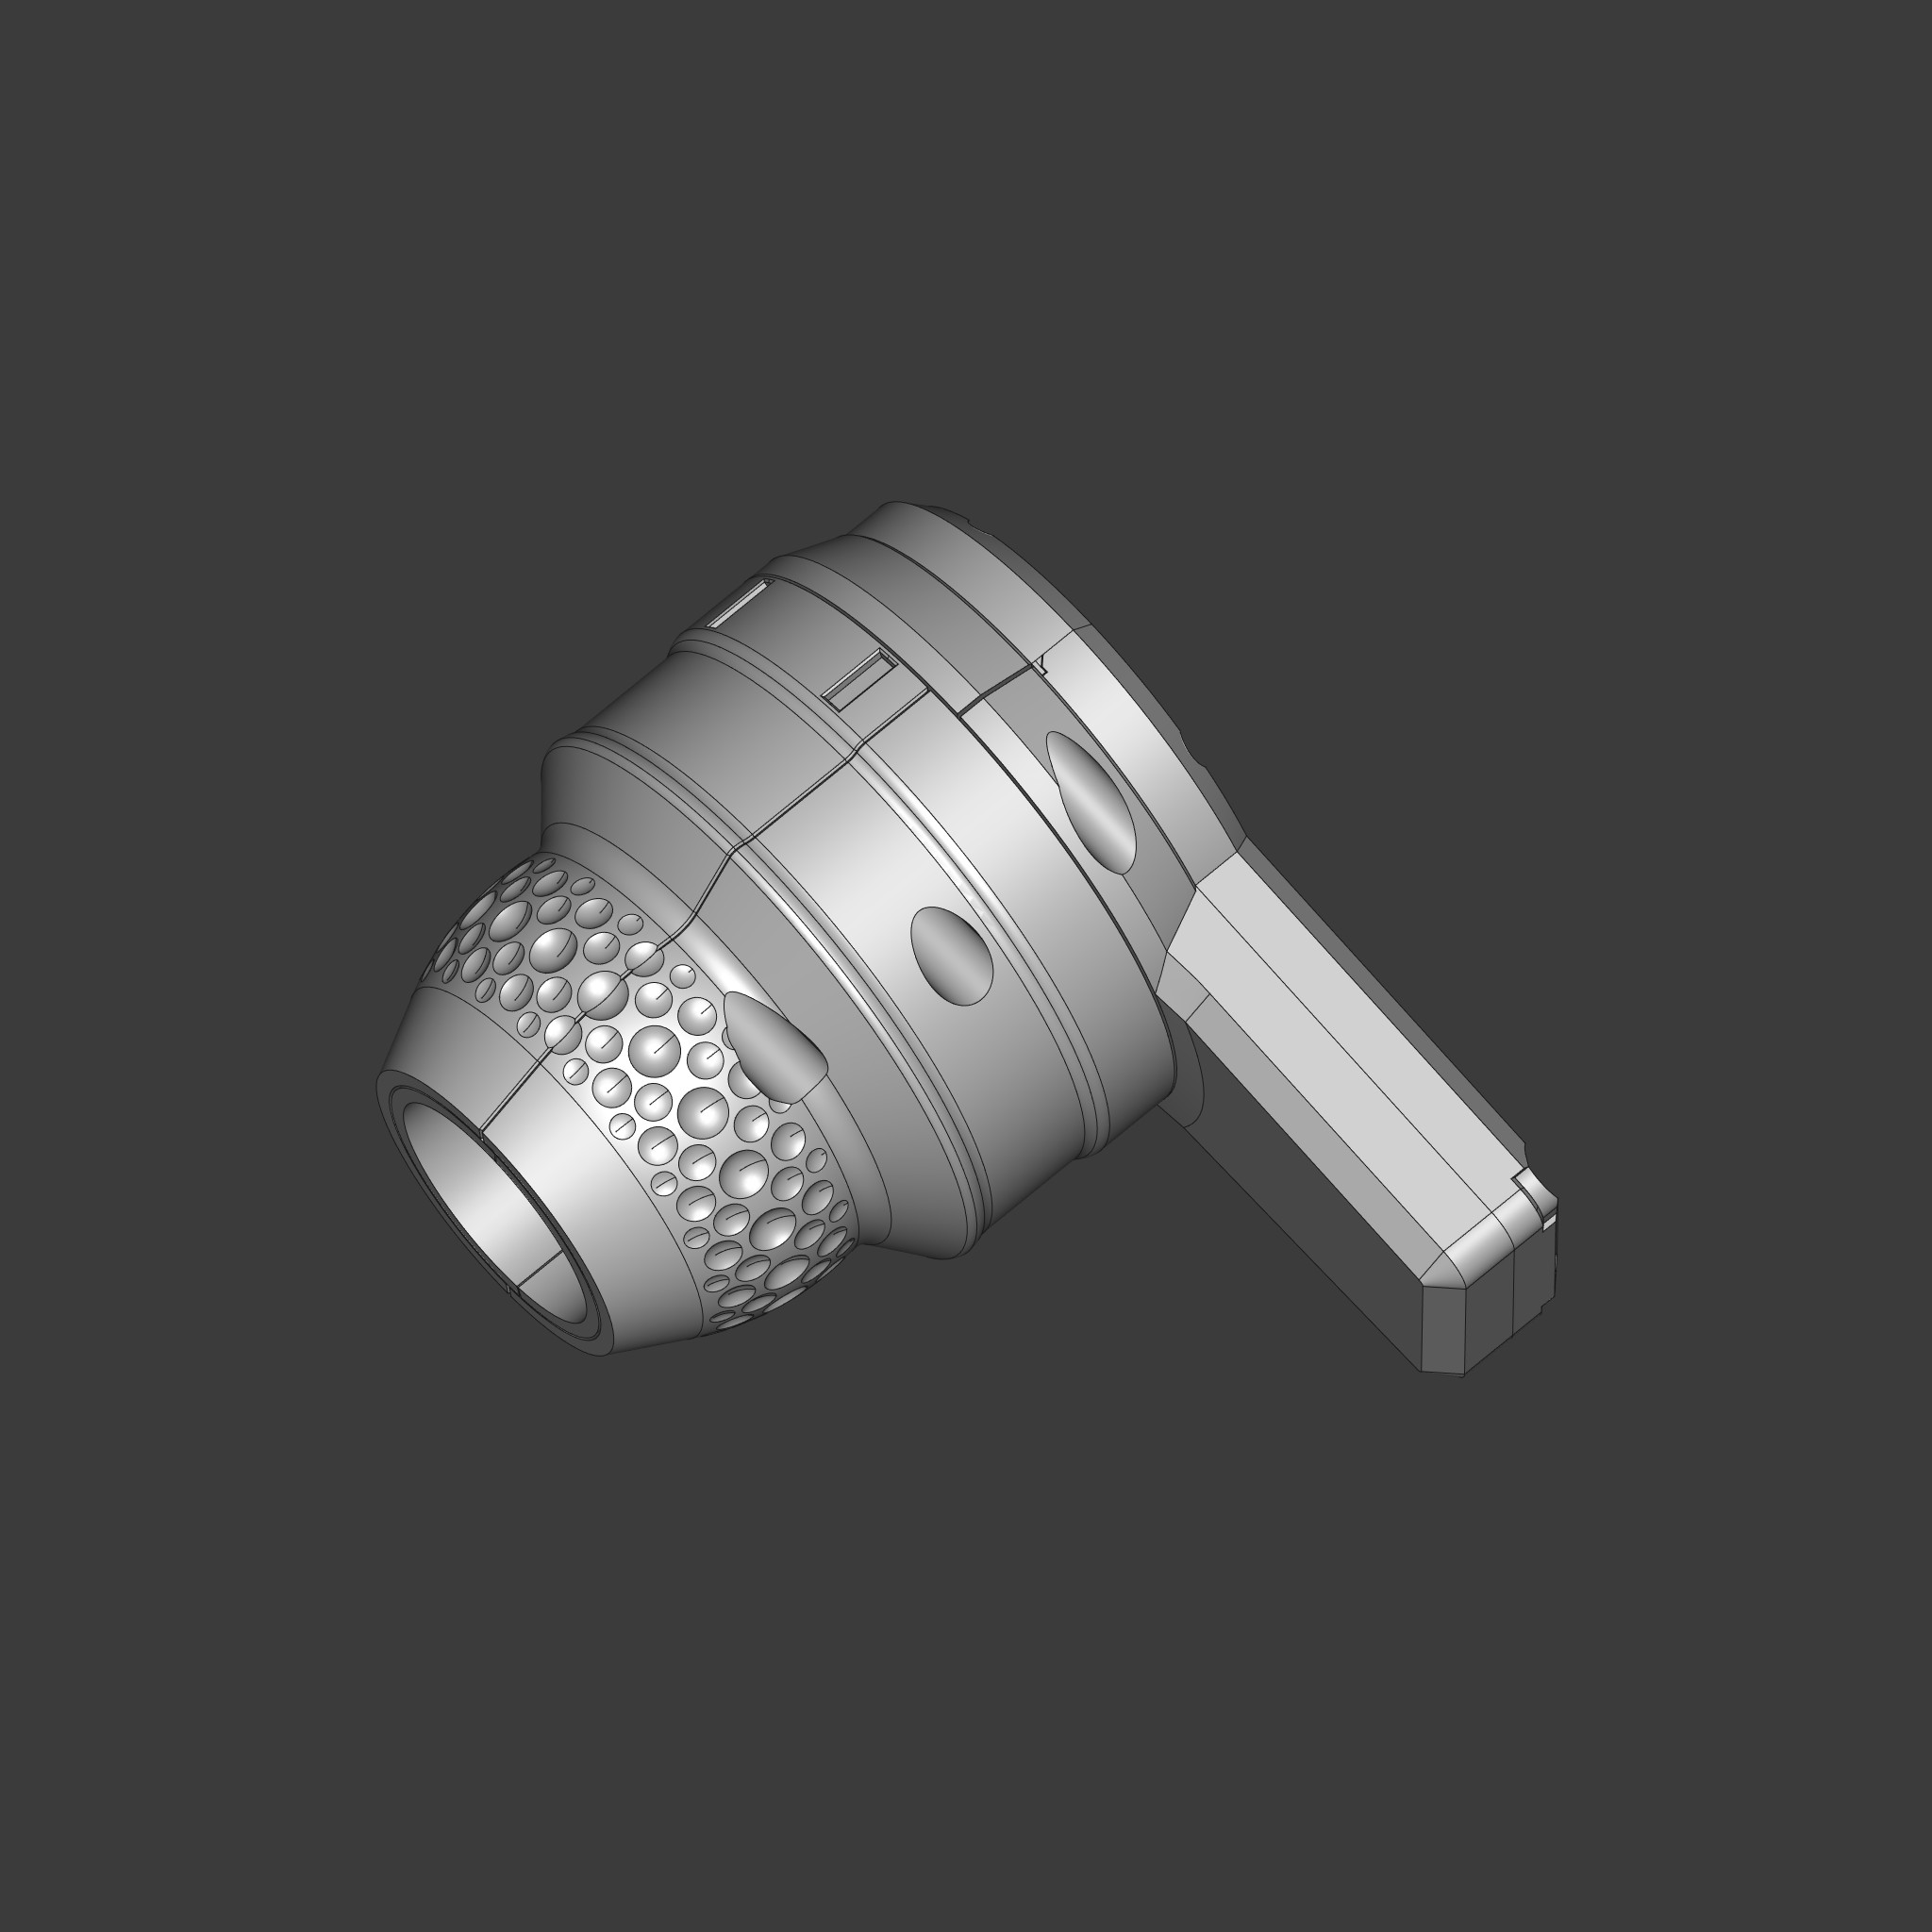
\includegraphics[width=.9\linewidth]{images/likertshift_freecad.jpg}
        \caption{CAD model}
    \end{subfigure}%
    \begin{subfigure}{.3333\textwidth}
        \centering
        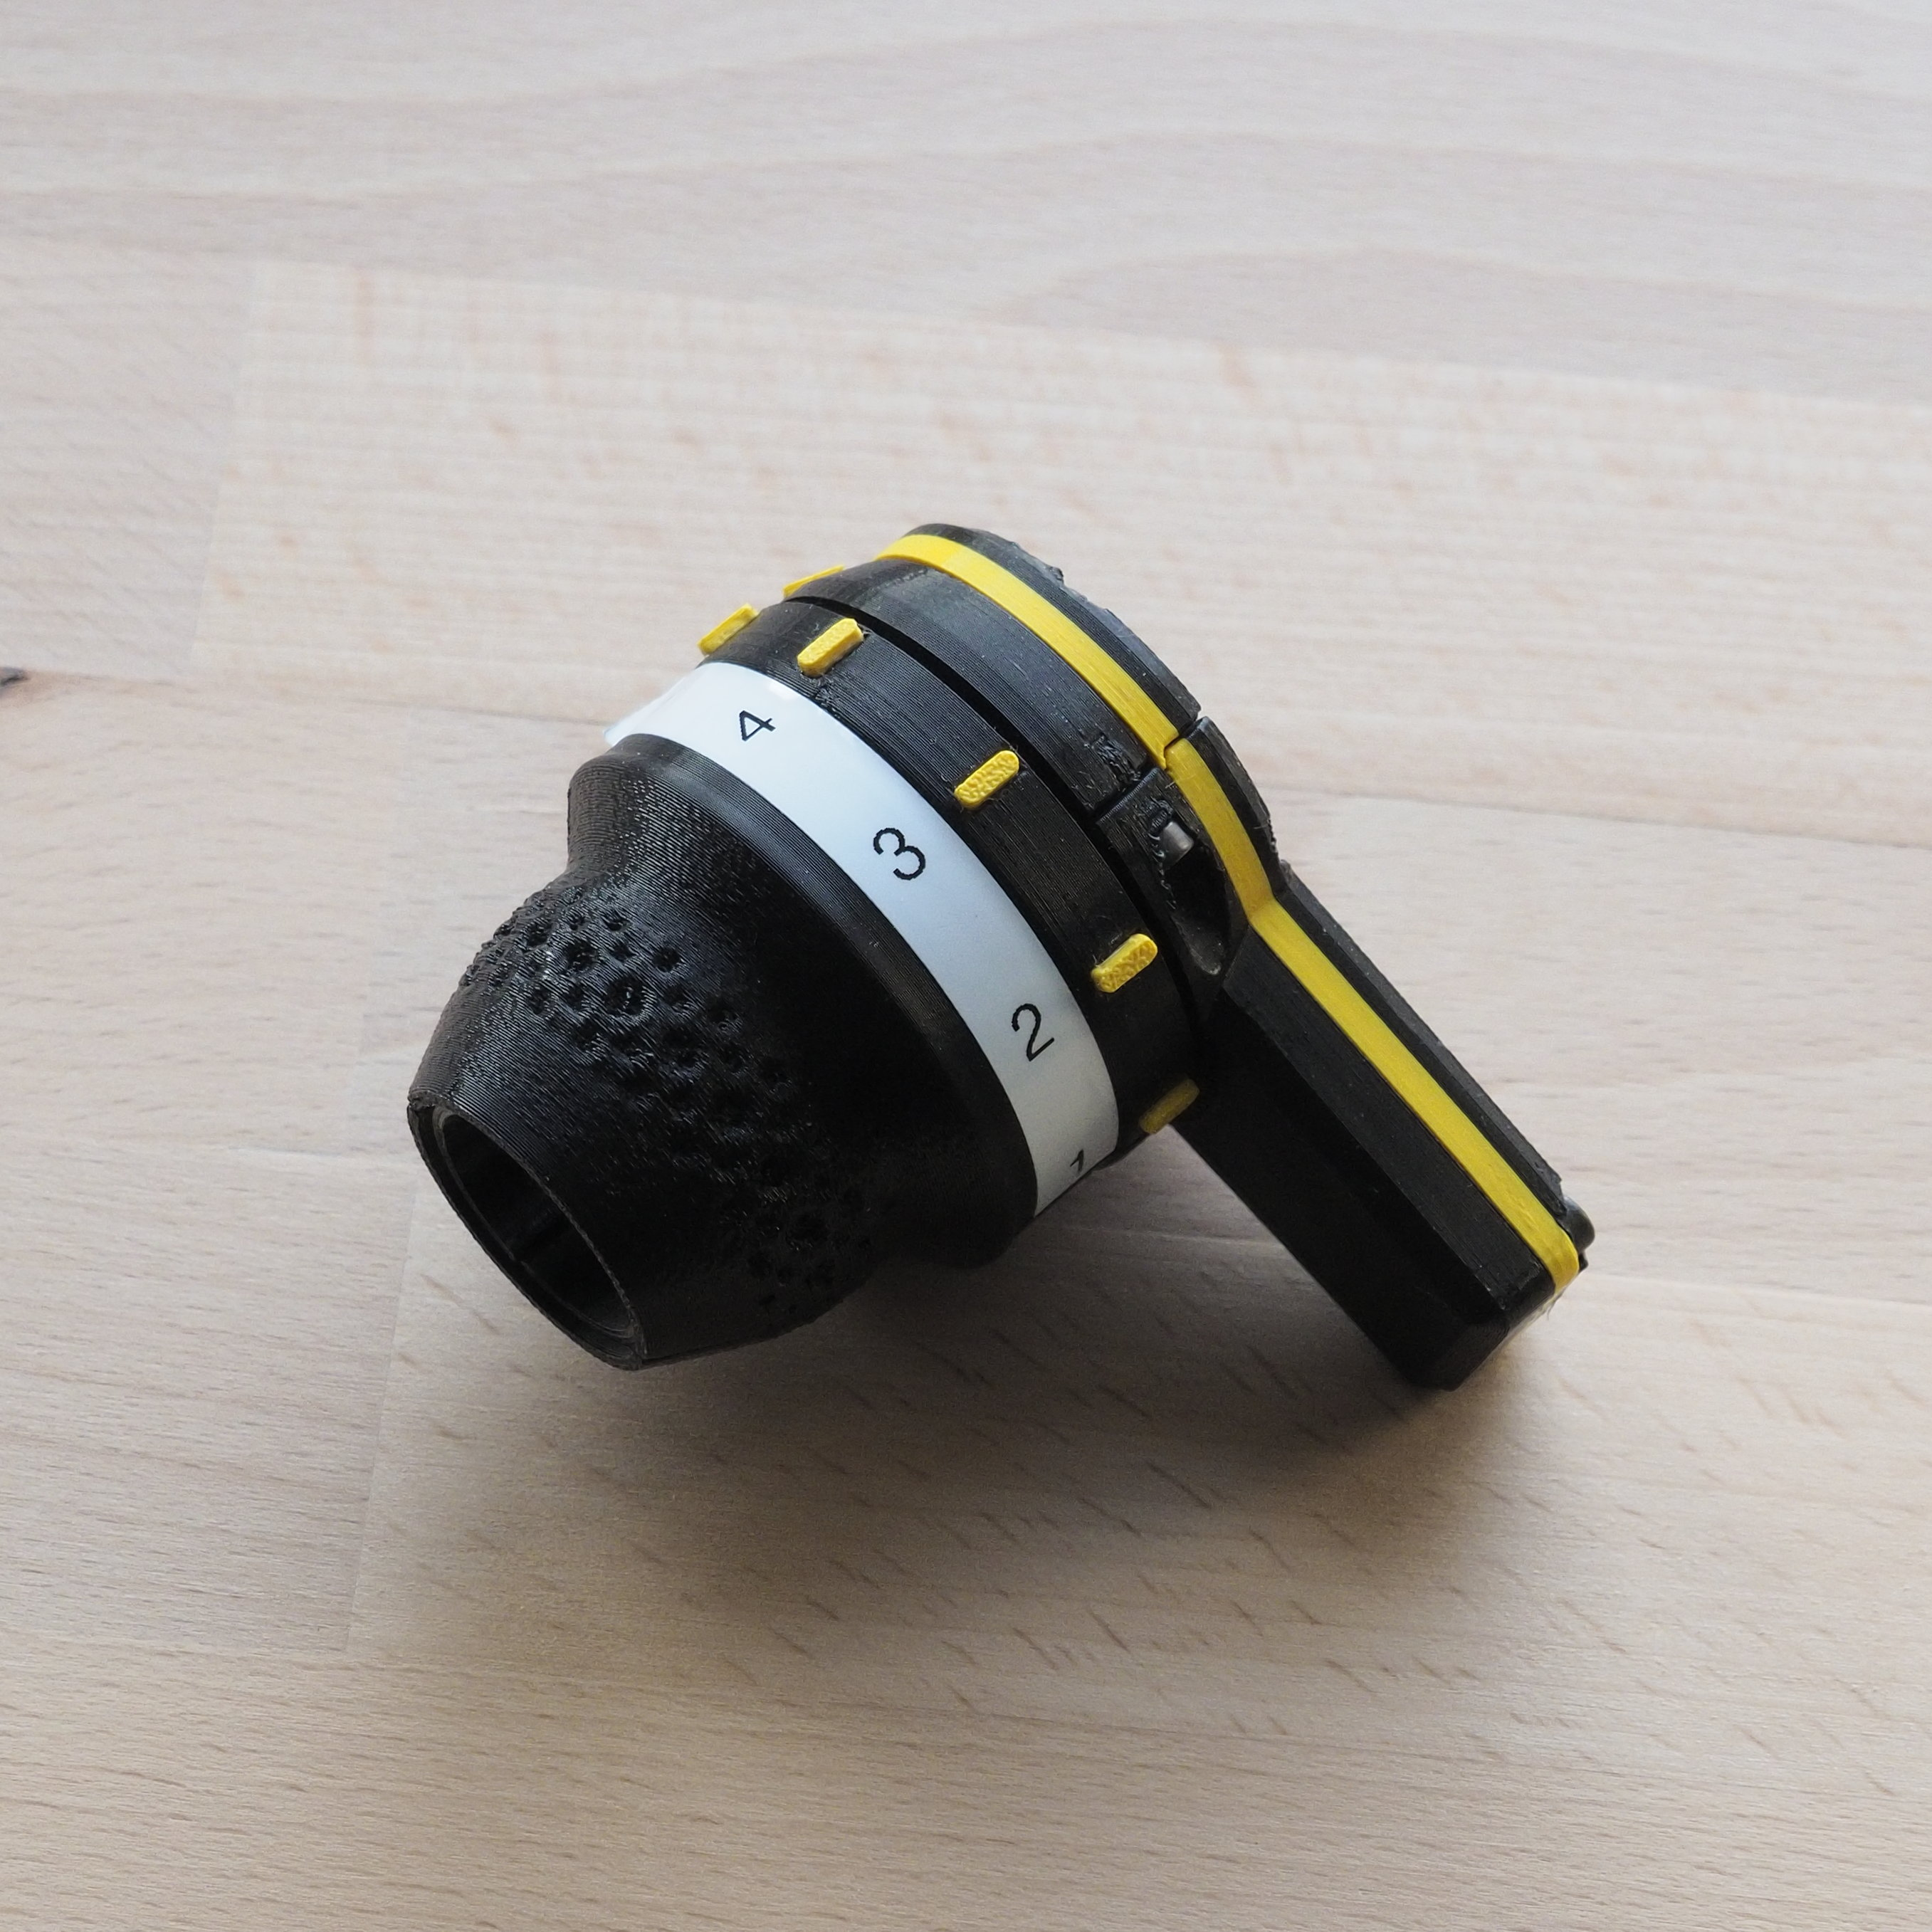
\includegraphics[width=.9\linewidth]{images/likertshift_assembled.jpg}
        \caption{Fully assembled}
    \end{subfigure}%
    \begin{subfigure}{.3333\textwidth}
        \centering
        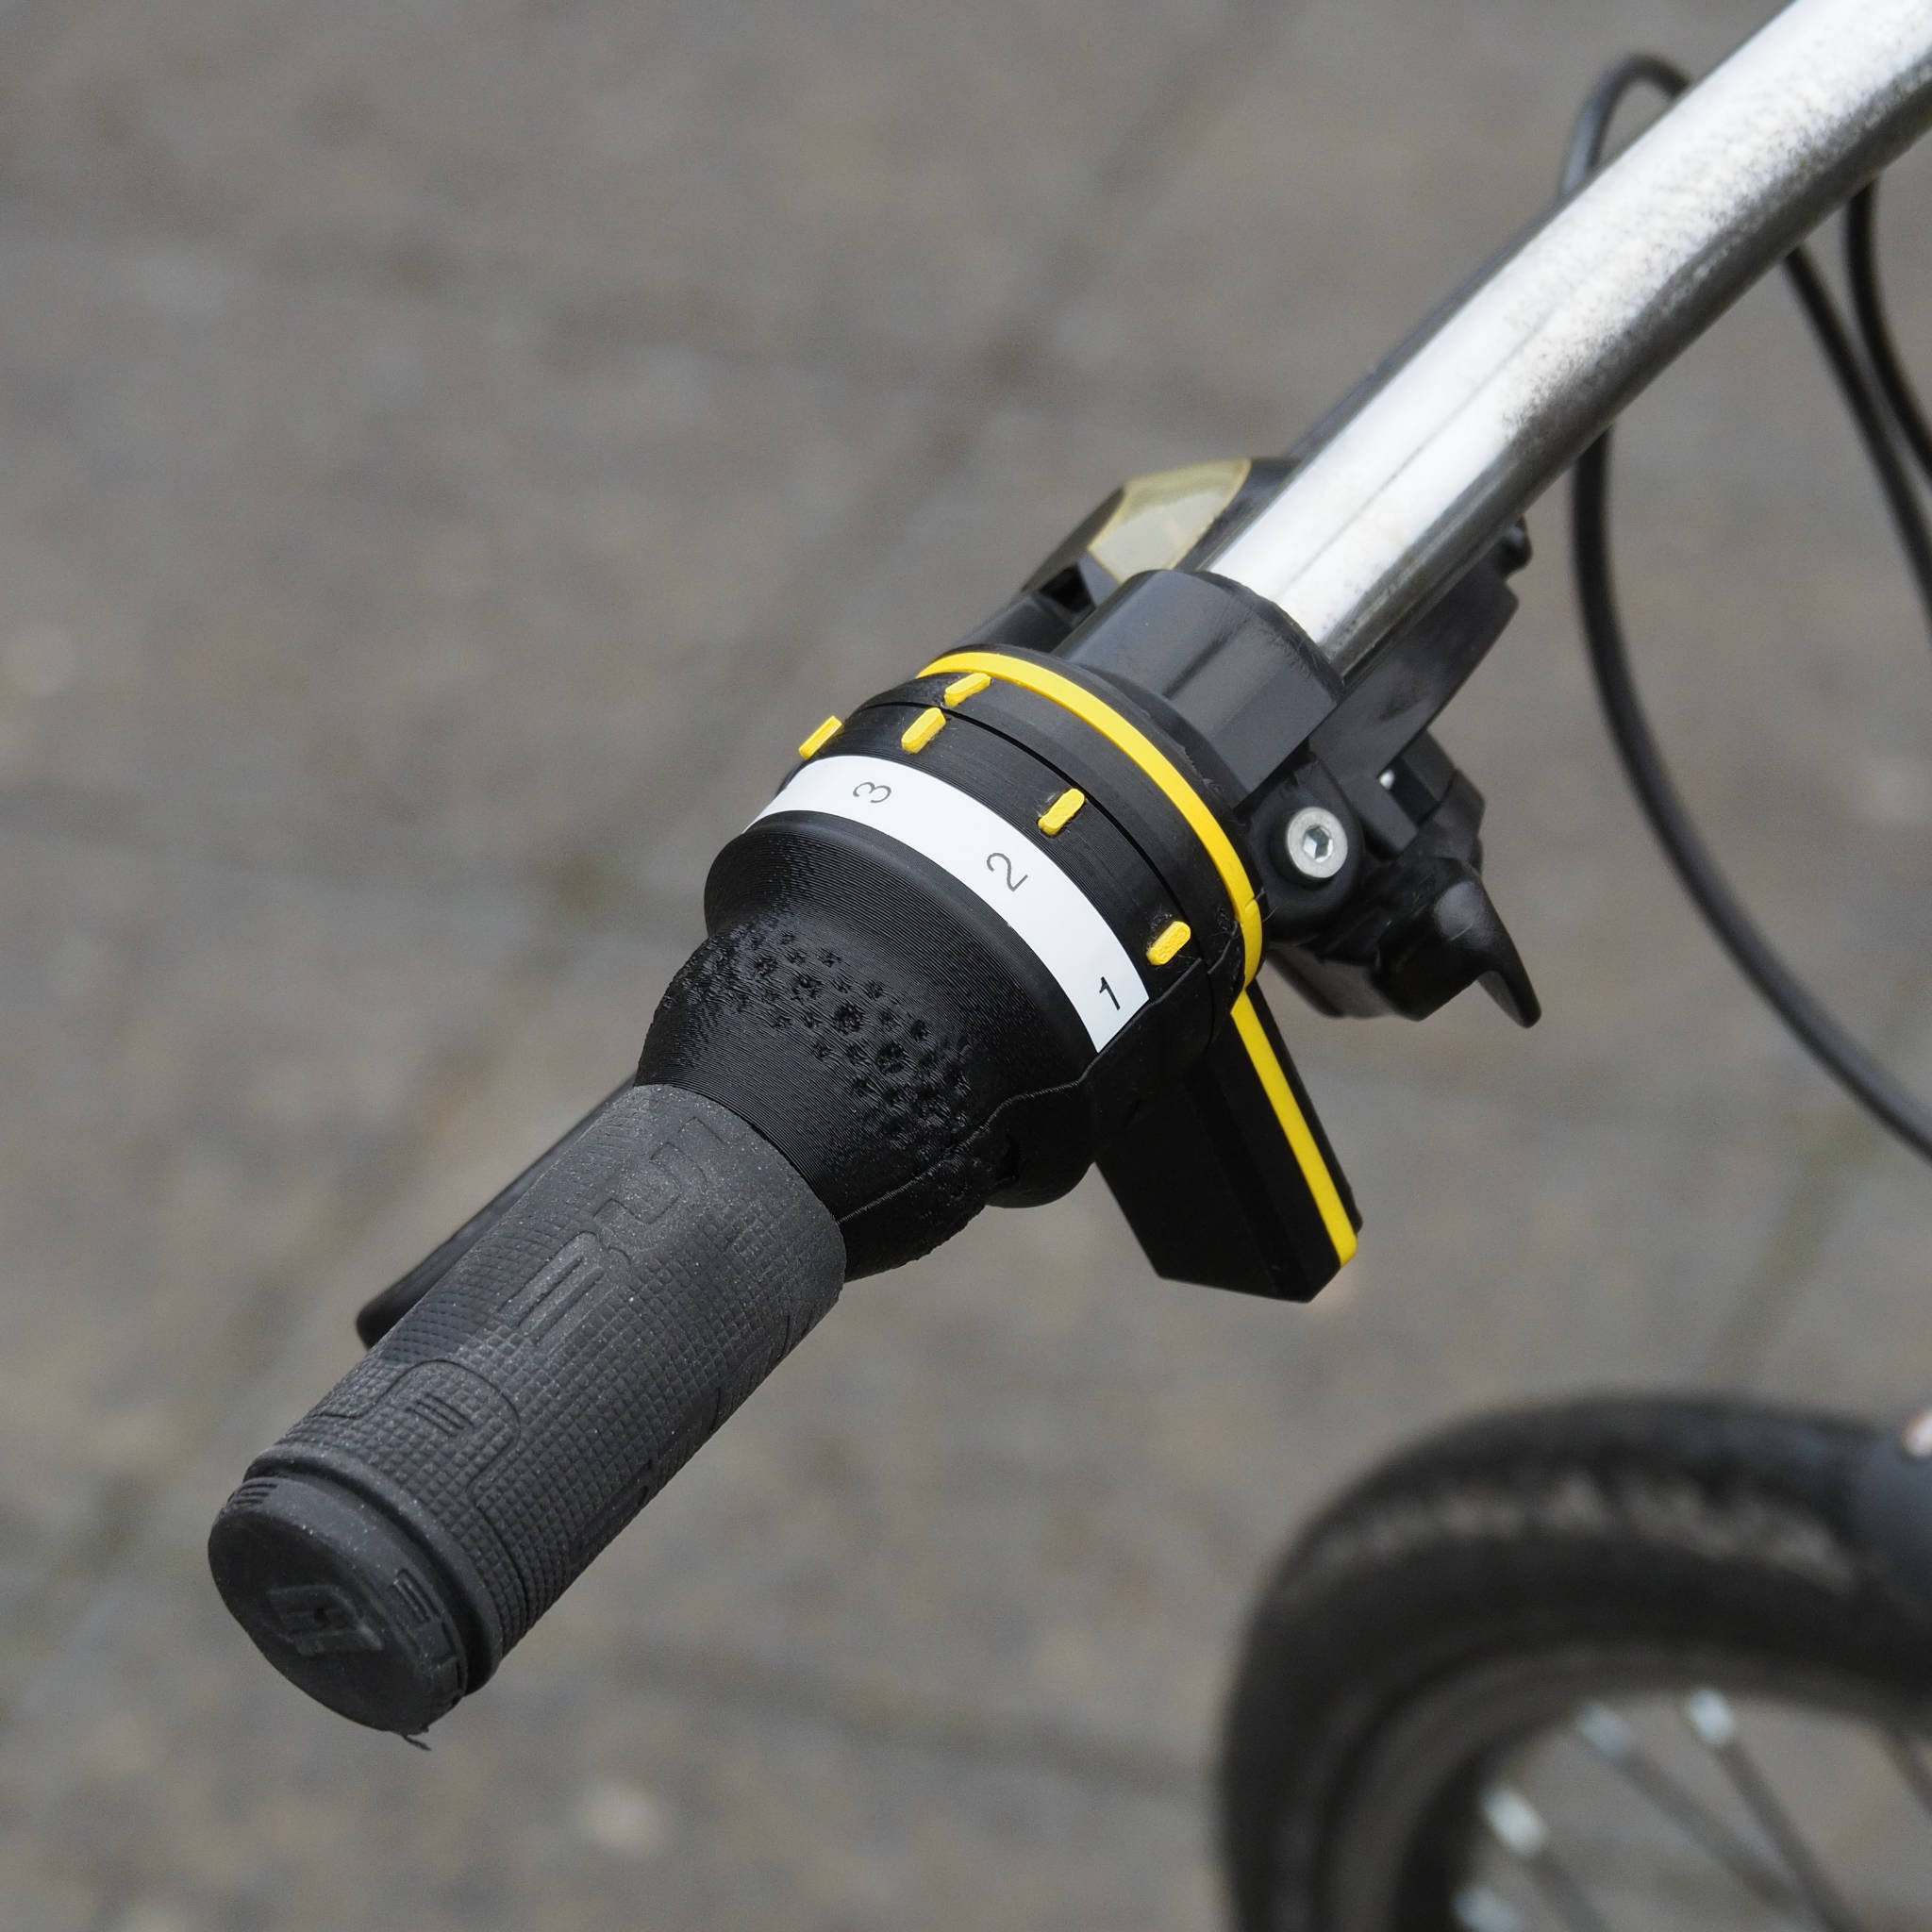
\includegraphics[width=.9\linewidth]{images/likertshift_mounted.jpg}
        \caption{Mounted to the handlebars}
        \label{subfig:likertshift_mounted}
    \end{subfigure}
    \caption{The final LikertShift prototype}
    \label{fig:likertshift}
\end{figure}

\noindent
To mount the prototype, the device is split in half and utilizes a simple clamping mechanism, similar to ones used for commercial bike accessories, to fix it to the handlebars.
We tried to add some texture to the clamping surface (see \autoref{subfig:cad_clamping_surface}), to reduce the necessary clamping pressure, but had mixed results with this.
The best solution to stop unwanted rotations and movements has been to apply a piece of masking tape to the handlebars at the desired mounting location.

We modeled a cavity to allow the application of a label sticker to mark the value of each discrete step and also added small markers to indicate the position that is currently selected.
The markers are 3D printed with a different filament color to improve visibility.
We also used a combination of CAD modeled indents, as well as the so-called “Fuzzy skin” feature in our slicer\footnoteurl{https://help.prusa3d.com/article/fuzzy-skin_246186} to add some texture to the grip area (see \autoref{subfig:slicer_textured_grip_area}).
This could be improved by utilizing multi-material 3D printing techniques and printing parts of it in more “grippy” materials like TPU, but we decided against such an approach, because multi-material 3D printing either requires special multi-toolhead printers or generates a lot of wasted material.

To satisfy \ref{drq:robust} and \ref{drq:easy_to_reproduce} we designed the device to be fully integrated, without requiring any external power.
\autoref{subfig:cad_pcb_compartment} shows the electronics compartment which houses the main Microcontroller board, as well as a button-cell battery to supply power to the electronics (see \autoref{subsec:electronics}).

\begin{figure}[!htb]
    \centering
    \begin{minipage}{.3333\textwidth}
        \centering
        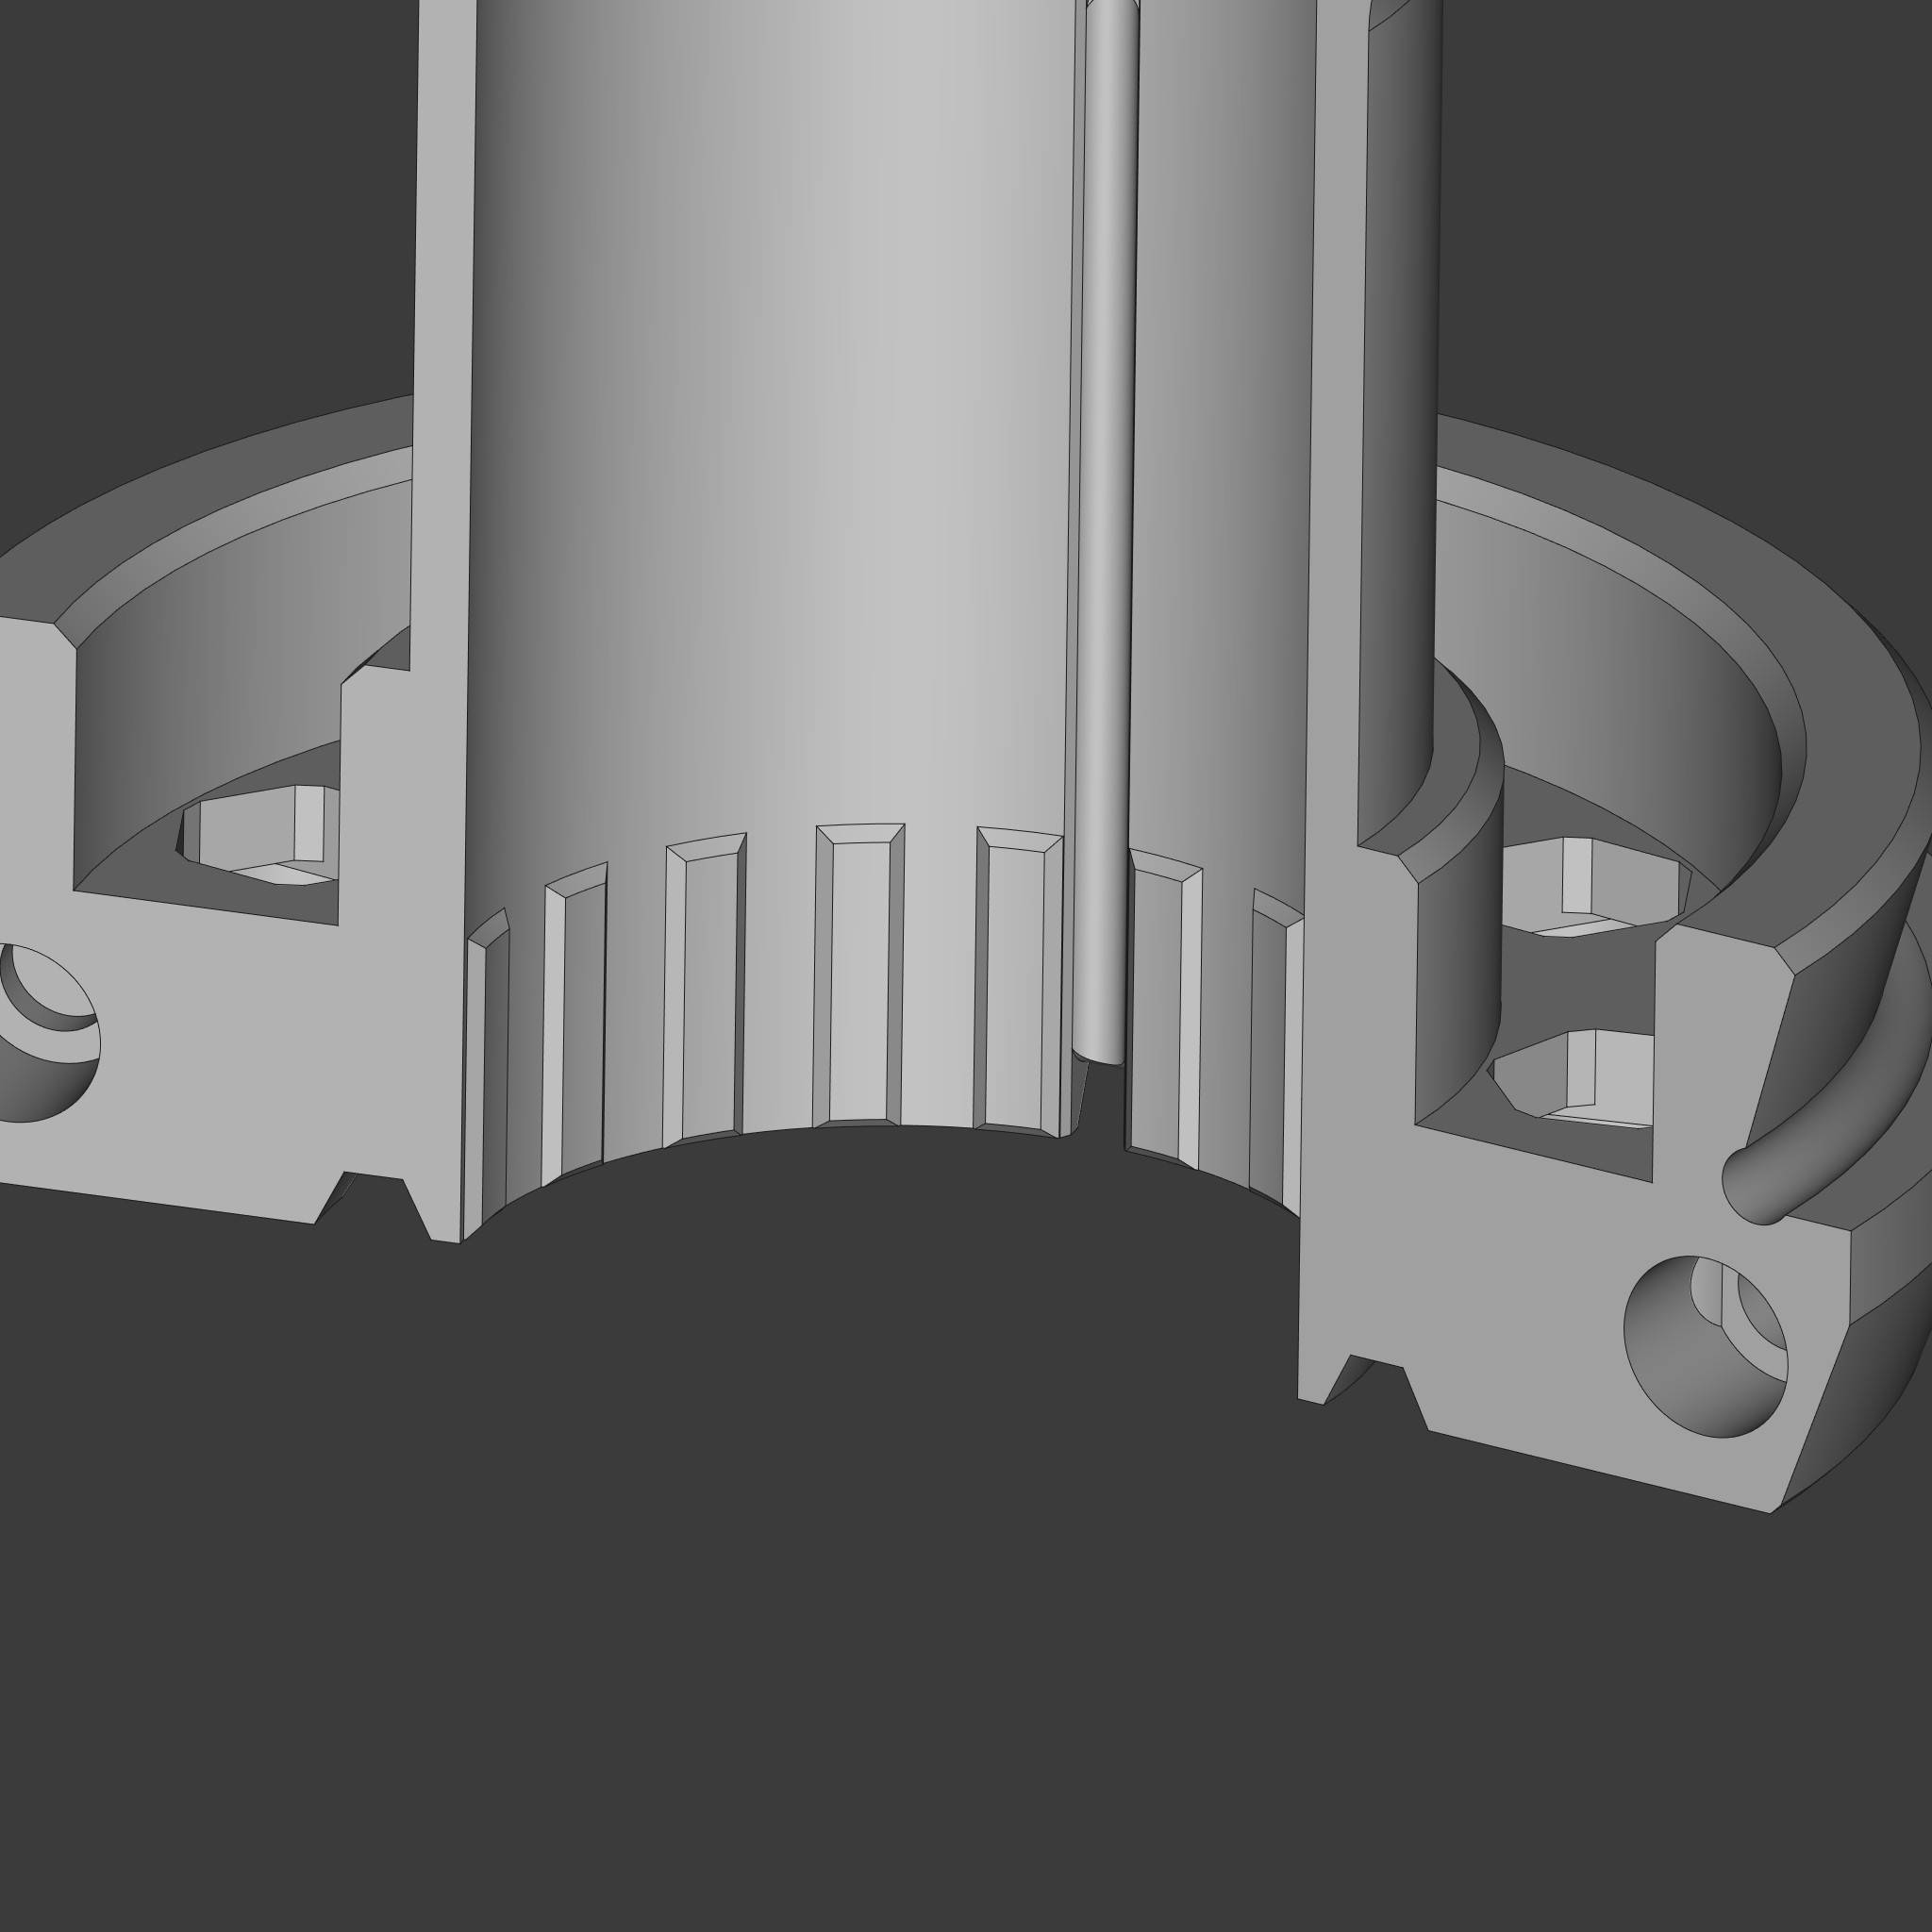
\includegraphics[width=.9\linewidth]{images/cad_clamping_surface.jpg}
        \caption{Clamping surface}
        \label{subfig:cad_clamping_surface}
    \end{minipage}%
    \begin{minipage}{.3333\textwidth}
        \centering
        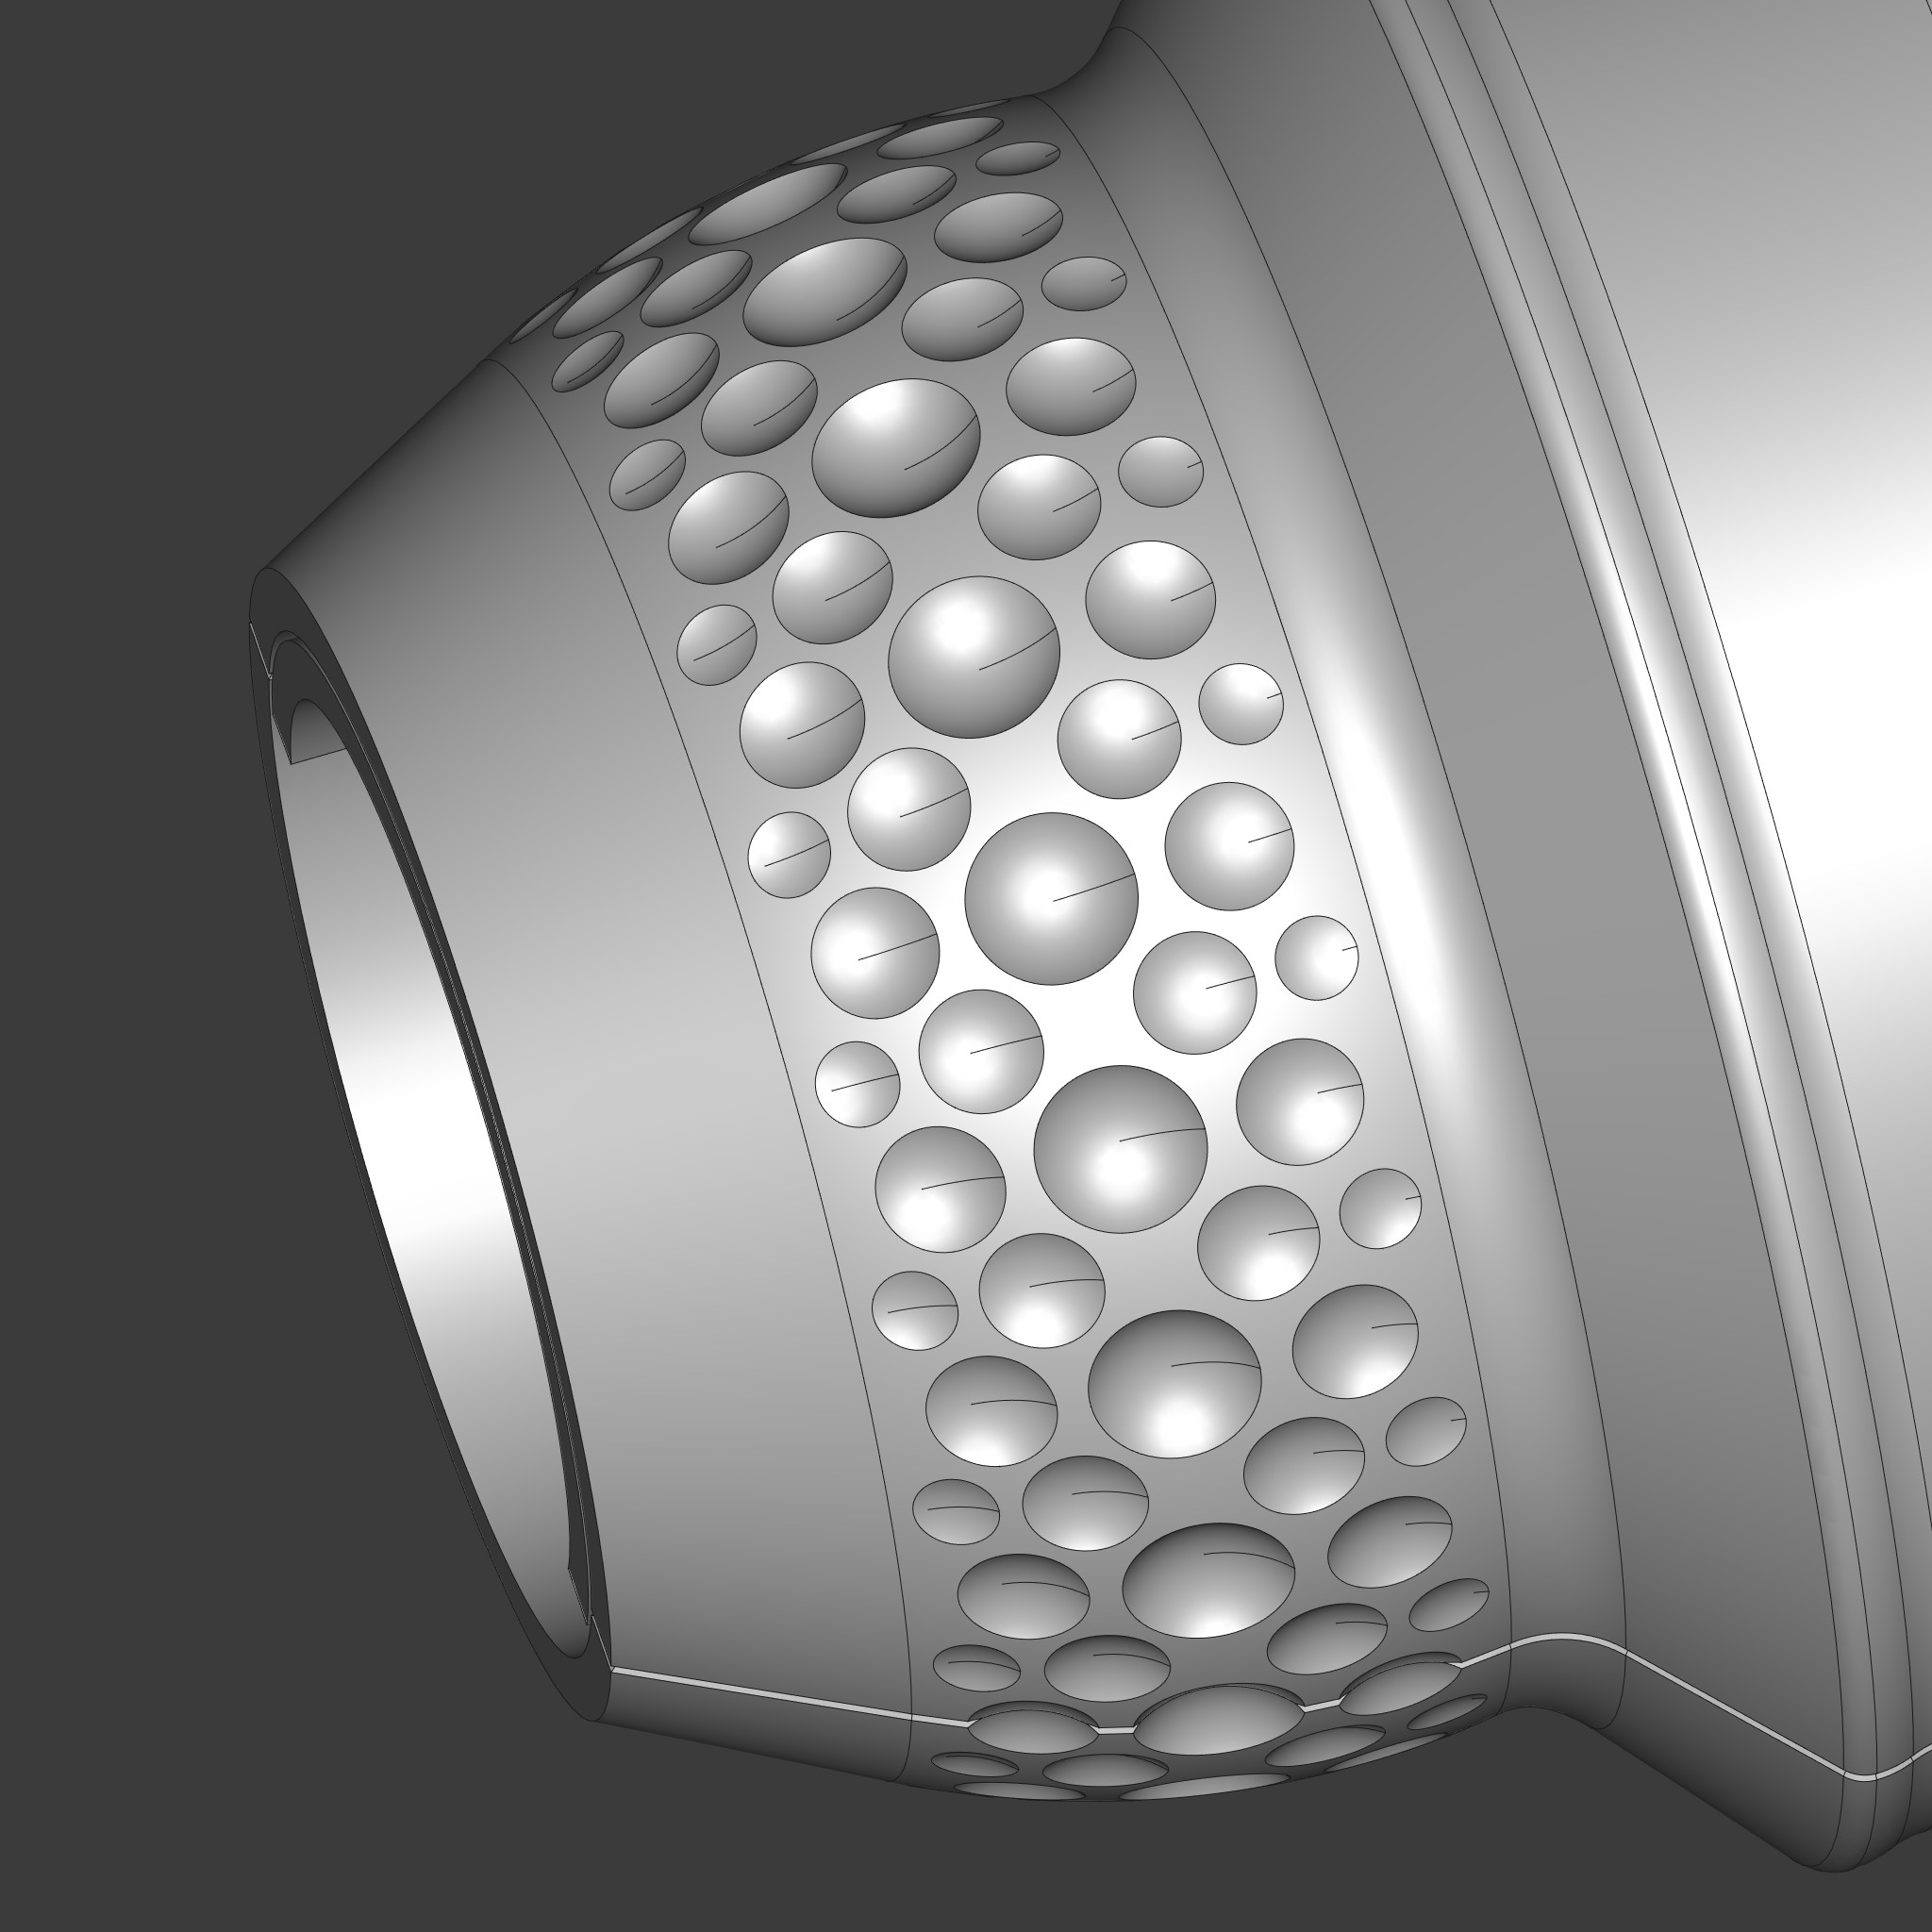
\includegraphics[width=.9\linewidth]{images/cad_grip_texture.jpg}
        \caption{Grip area}
        \label{subfig:slicer_textured_grip_area}
    \end{minipage}%
    \begin{minipage}{.3333\textwidth}
        \centering
        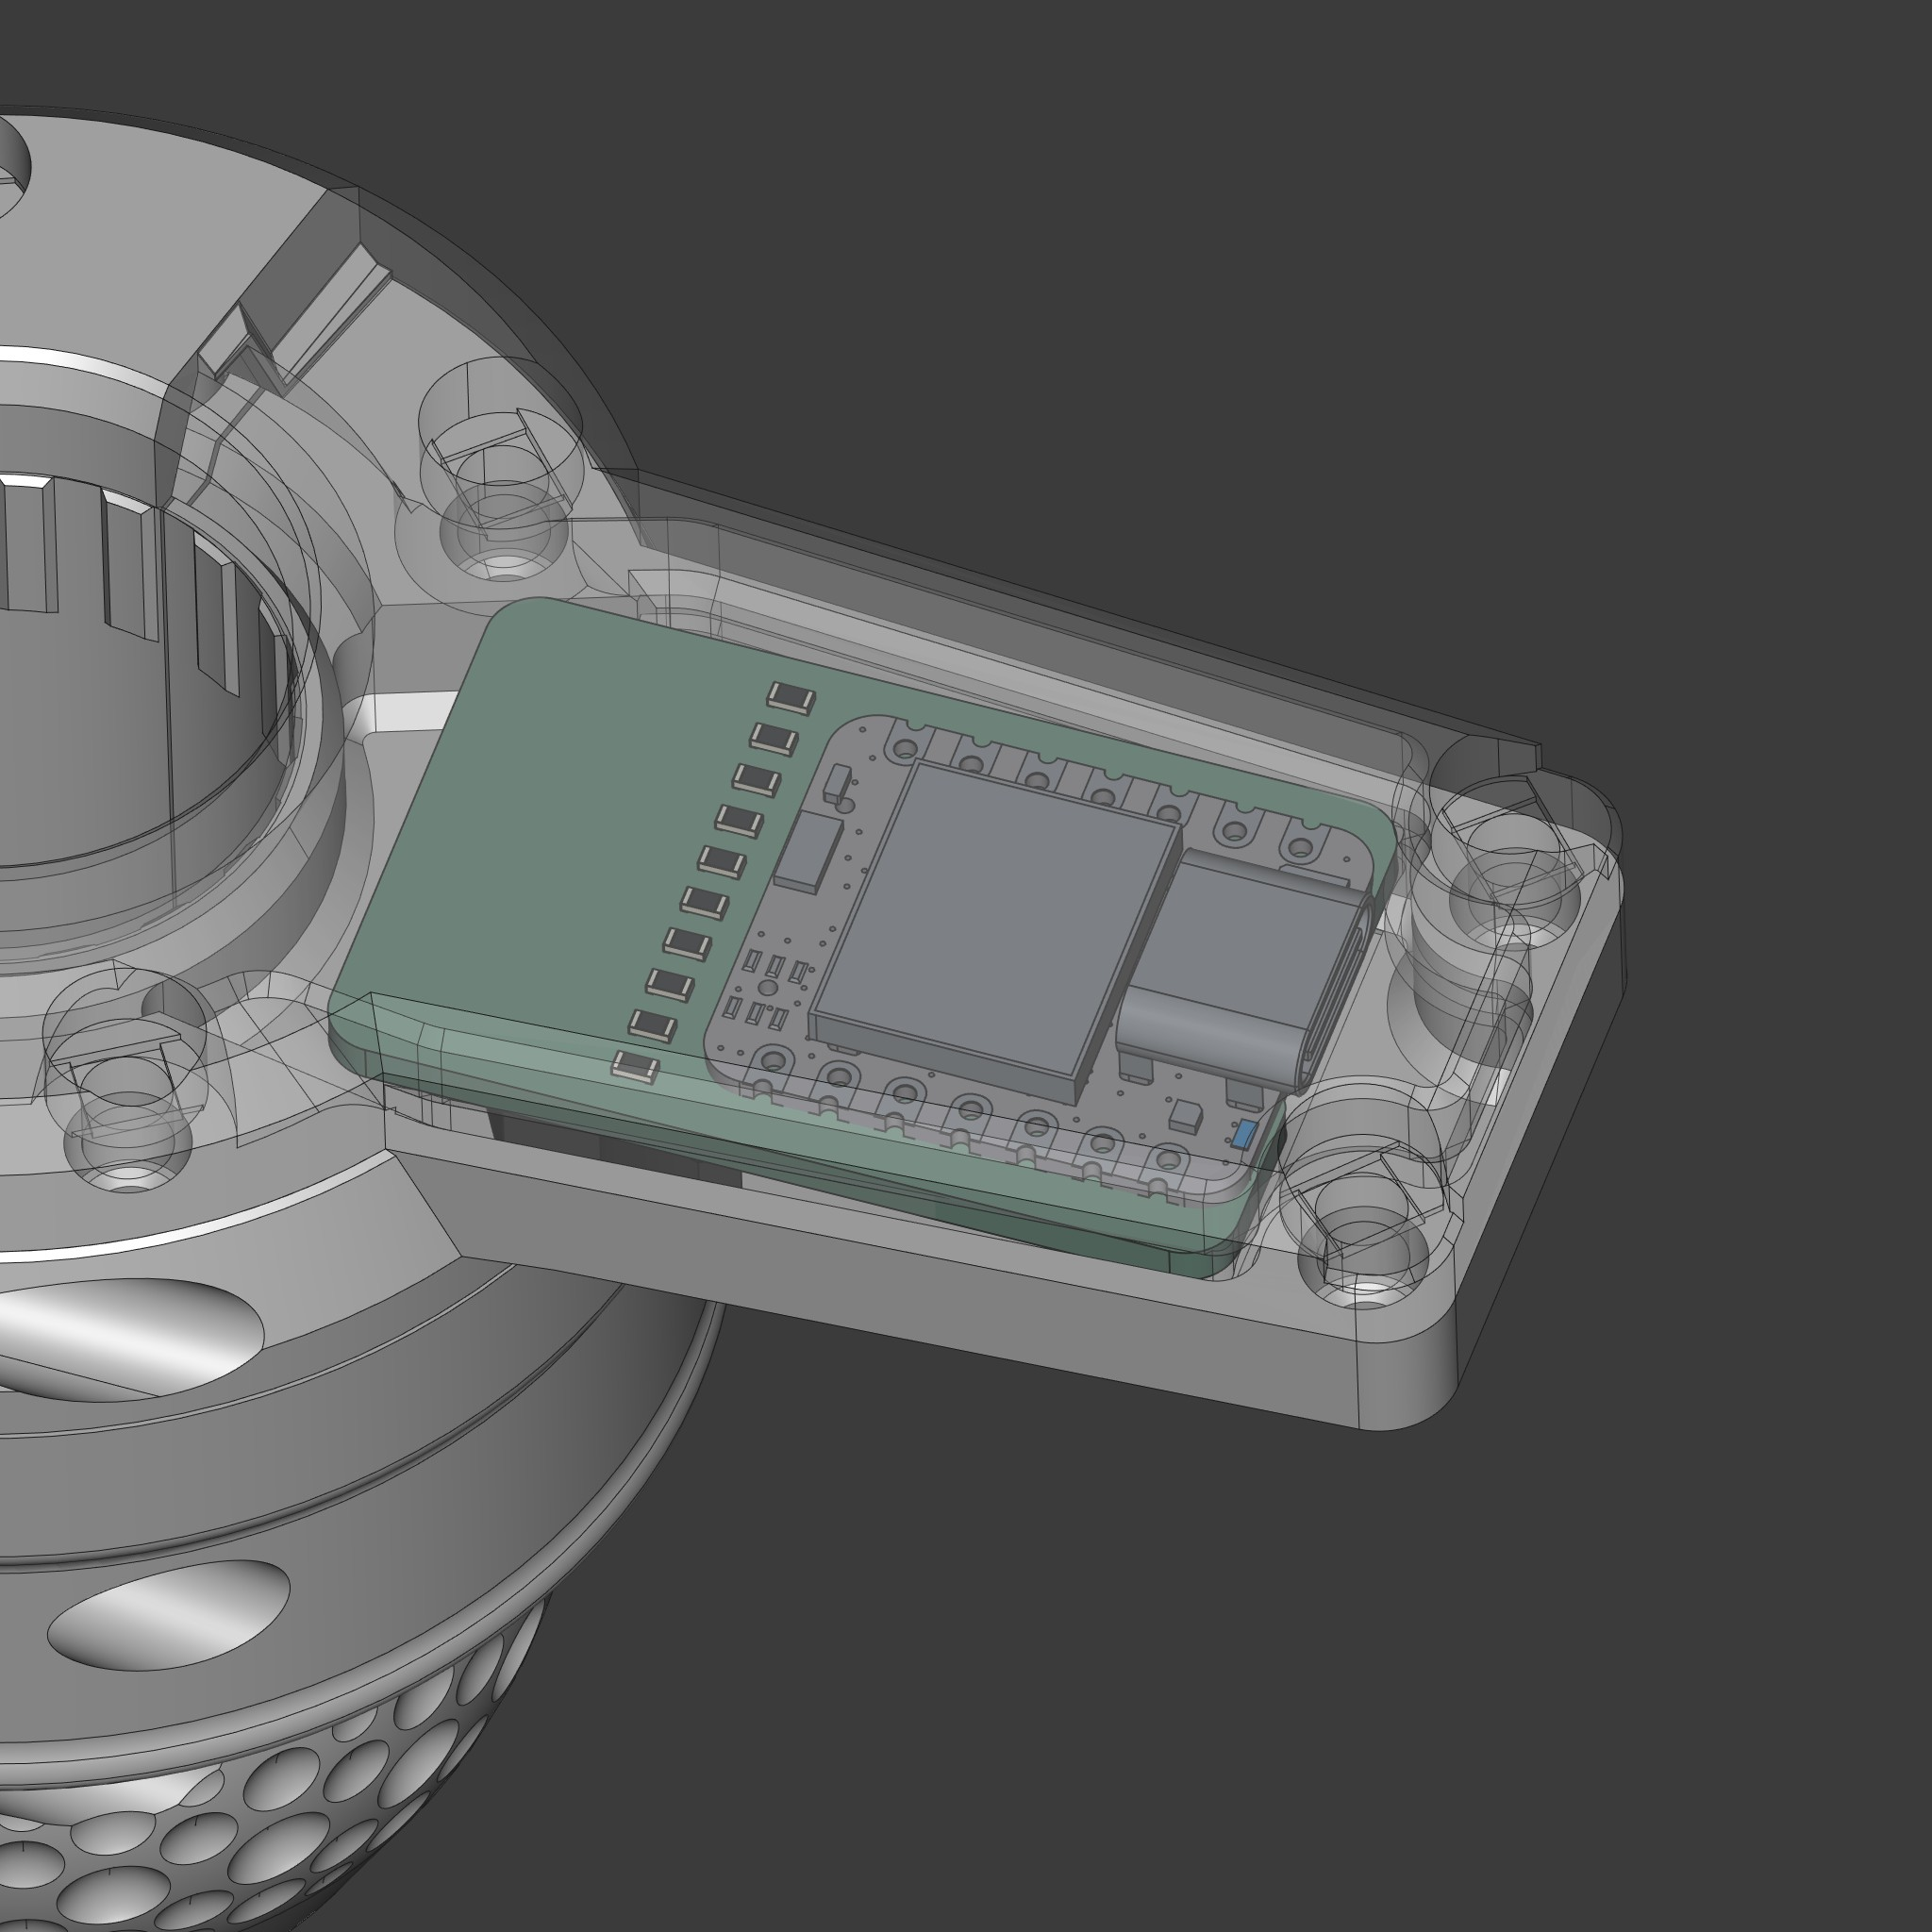
\includegraphics[width=.9\linewidth]{images/cad_pcb_compartment.jpg}
        \caption{PCB compartment}
        \label{subfig:cad_pcb_compartment}
    \end{minipage}
\end{figure}

\noindent
We used FreeCAD\footnoteurl{https://www.freecad.org/} (a parametric modelling software) in combination with OpenSCAD\footnoteurl{https://openscad.org/} (a code-based solid modelling software) for the mechanical design of our prototype. Both programs qualify as free and open-source software (FOSS), ensuring the design is accessible and modifiable by future contributors without requiring expensive software licenses.
The design was created parametrically, allowing for parameters like the number of discrete positions or their spacing to be easily adjusted.
All parts have been designed specifically for FDM 3D printing, with a particular print orientation in mind and don't require any additional support structures when printing.

\subsubsection{Mechanism}\label{subsec:mechanism}

\def\rotator{\textsf{Rotator}\xspace}
\def\rotatorhead{\textsf{Rotator-head}\xspace}

The prototype uses a simple rotary switching mechanism.
When the outer \rotator gets rotated, it pulls the \rotatorhead along a ramped track (see \autoref{fig:cad_ramped_track}).
The \rotatorhead, shown in \autoref{fig:cad_rotator_head}, consists of a \SI{4}{mm} steel bearing ball that is socketed into a 3D printed part and gets pushed into the track by a spring.
It is constrained to only move along the rotation axis by $\sim\SI{5}{\mm}$ to be able to overcome the ramps.
This way, the mechanism automatically snaps into the depressions between the ramps.

At the bottom of the depressions are nickel-plated neodymium magnets which are being used as the switching contacts while the \rotatorhead acts as the contactor.
M3 button head screws are used to clamp and connect cables to the contactor and switching contacts.
As the cable that goes to the \rotatorhead experiences lots of movement and thus relatively high stress, we used special FEP insulated wire\footnoteurl{https://shop.helukabel.com/de-en/heluflon-fep-6y-m25511/20271} made for the use in cable chains for it.
For the contacts we used standard PVC insulated wire.
This setup results in a total contact resistance of $\sim\SI{10}{\ohm}$, which is well within useable range for our purposes.

\begin{figure}[!htb]
    \centering
    \begin{minipage}{.3333\textwidth}
        \centering
        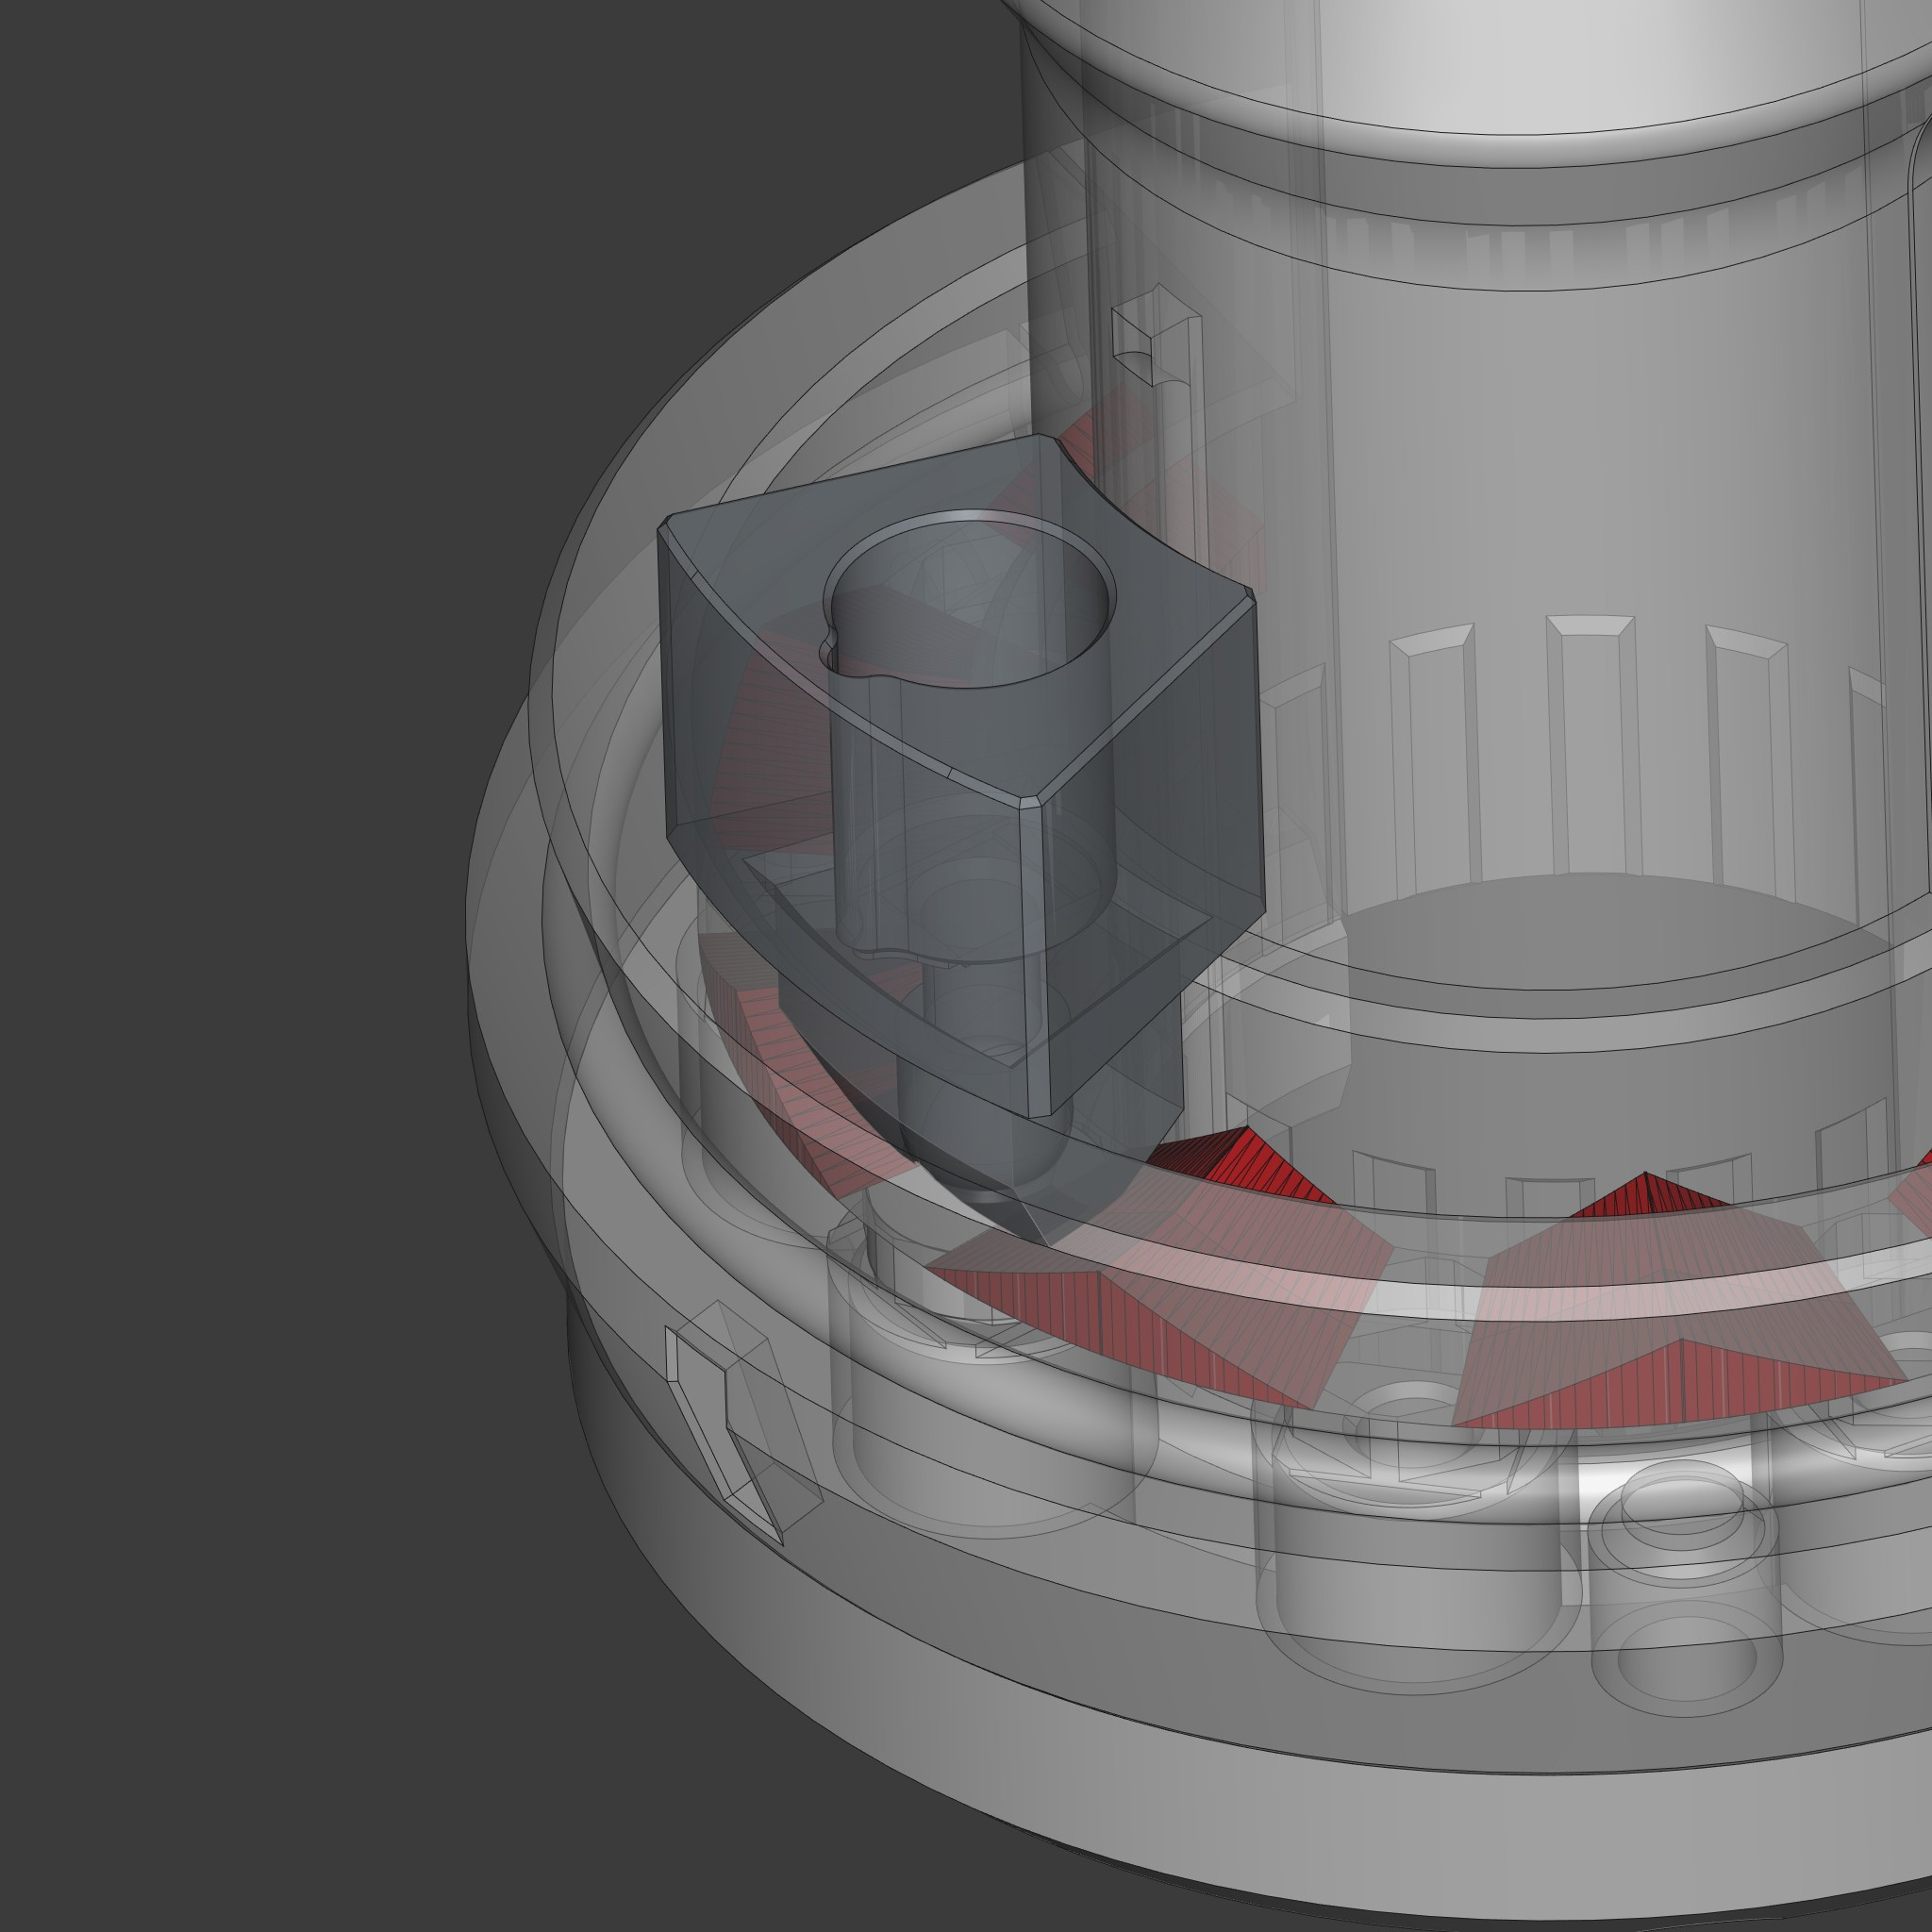
\includegraphics[width=.9\linewidth]{images/cad_ramped_track.jpg}
        \caption{Ramped track}
        \label{fig:cad_ramped_track}
    \end{minipage}%
    \begin{minipage}{.3333\textwidth}
        \centering
        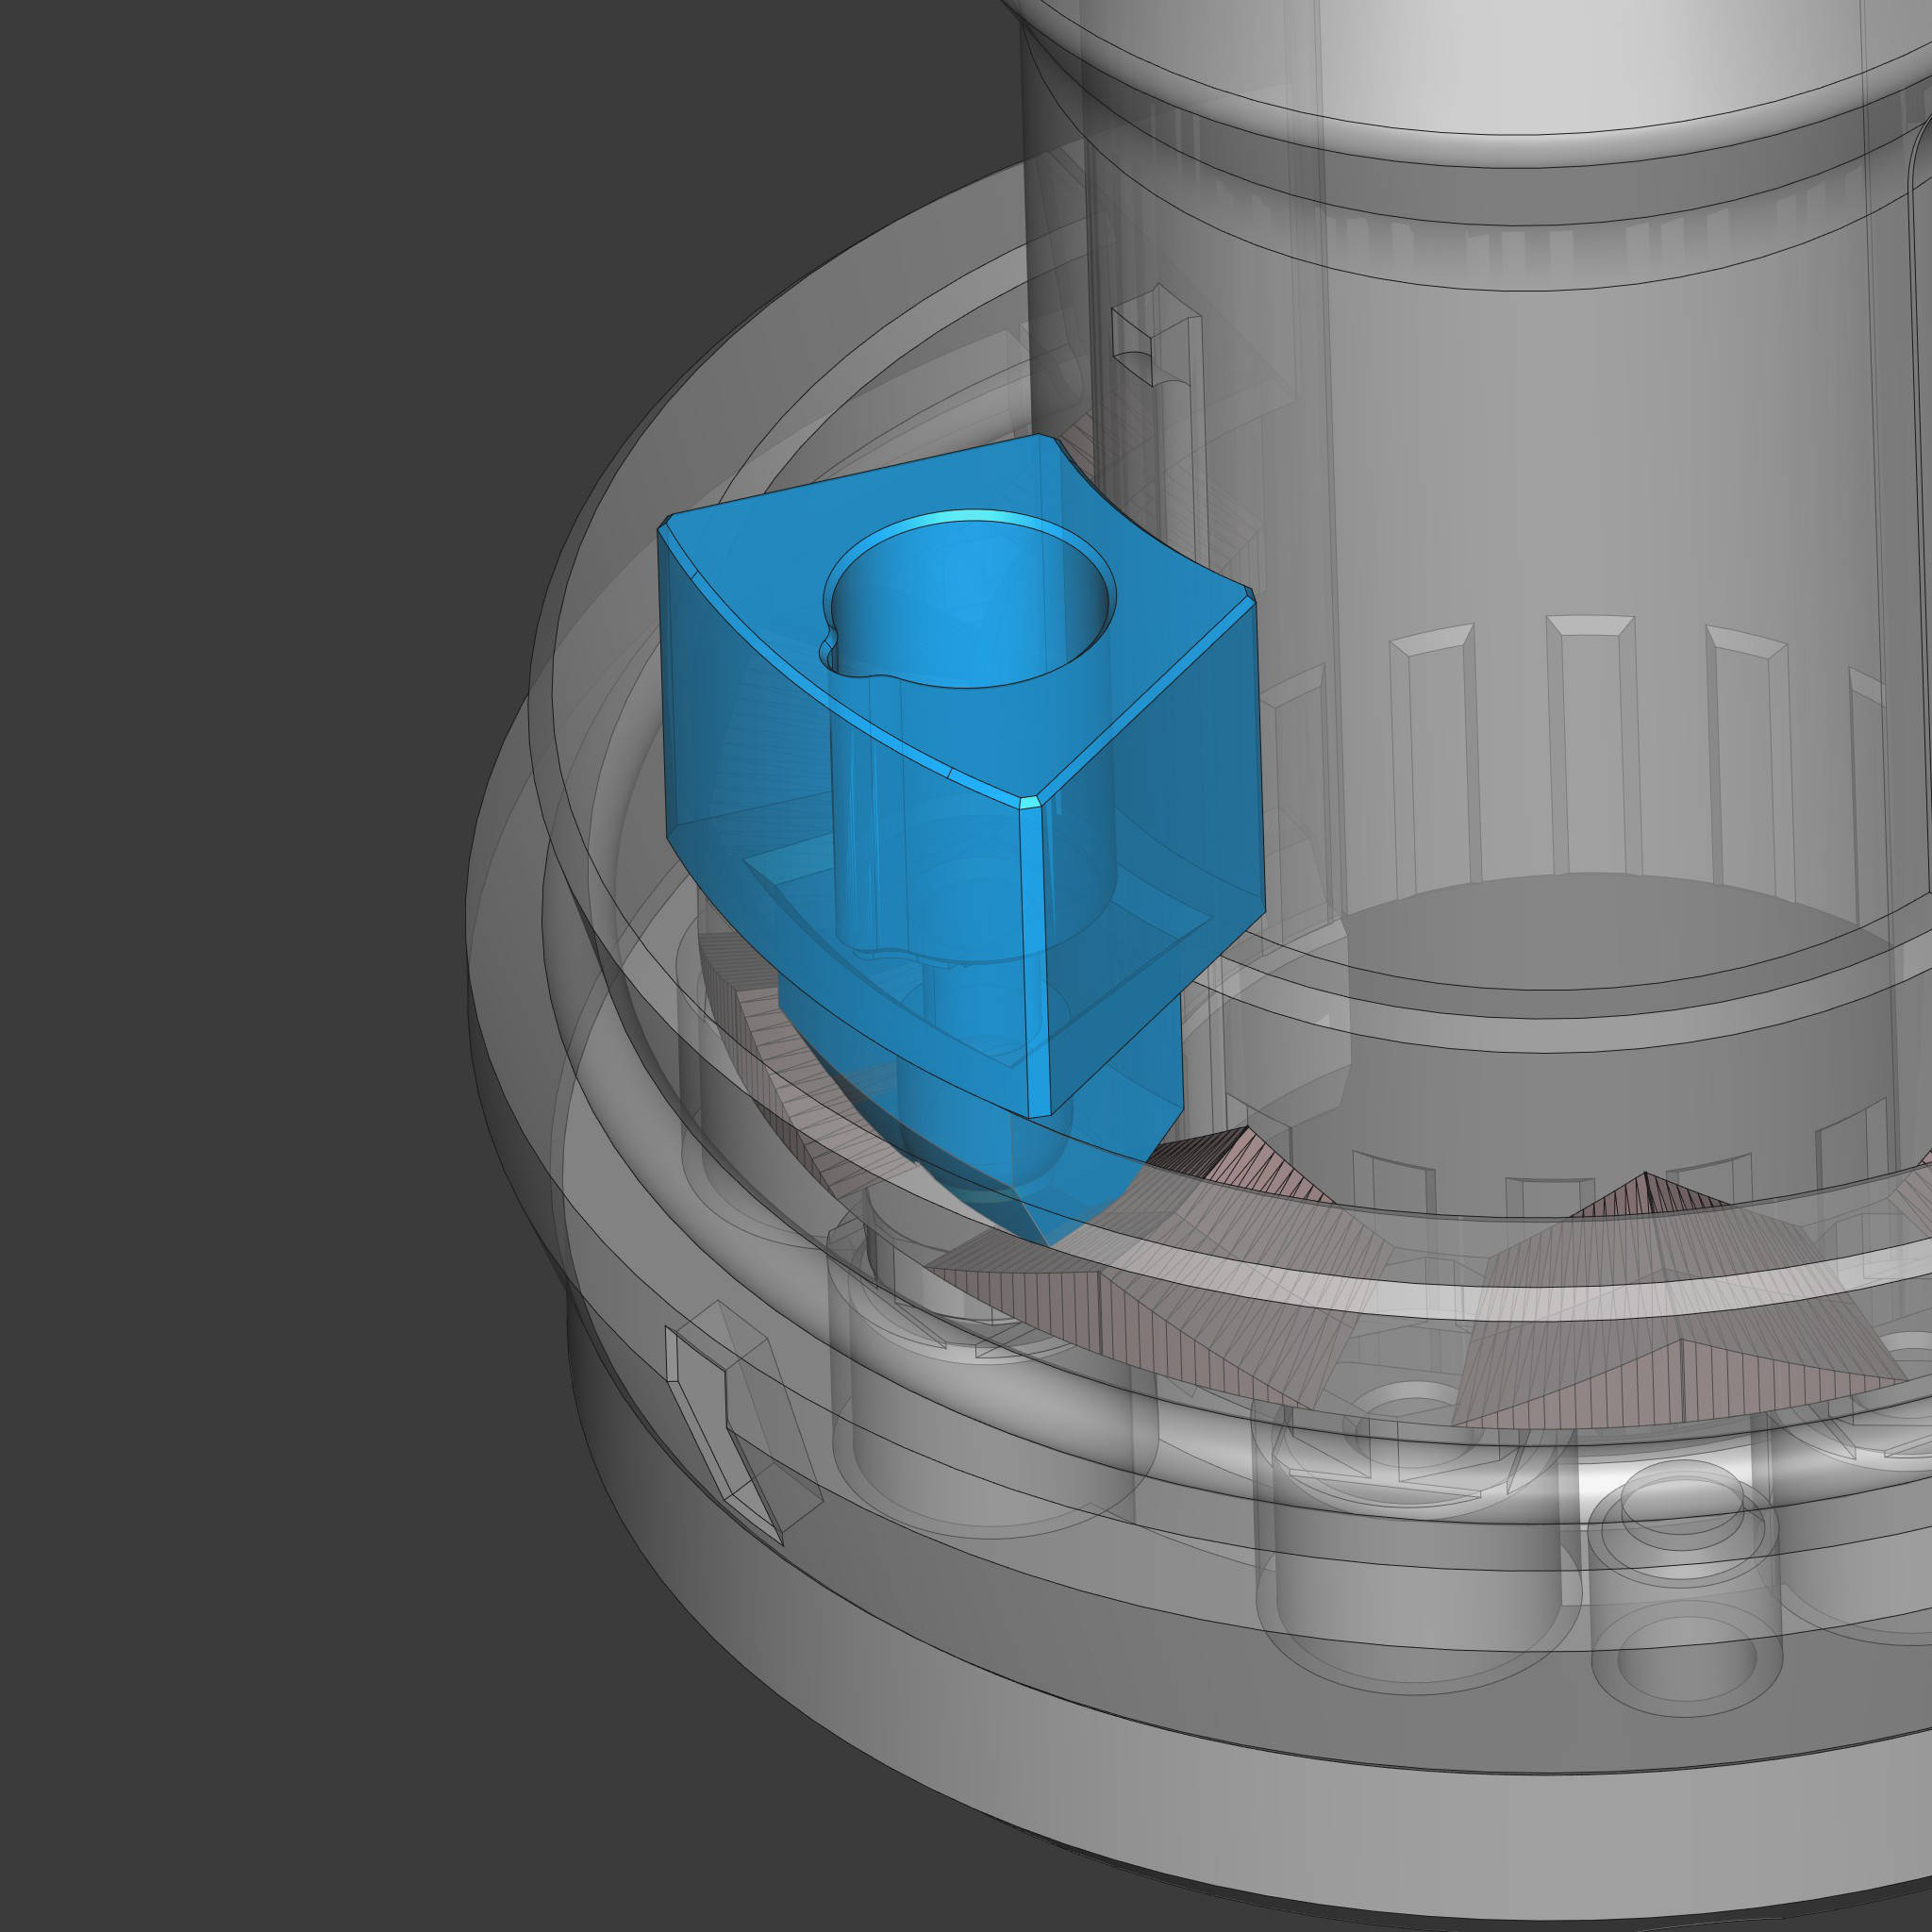
\includegraphics[width=.9\linewidth]{images/cad_rotator_head.jpg}
        \caption{\rotatorhead}
        \label{fig:cad_rotator_head}
    \end{minipage}%
    \begin{minipage}{.3333\textwidth}
        \centering
        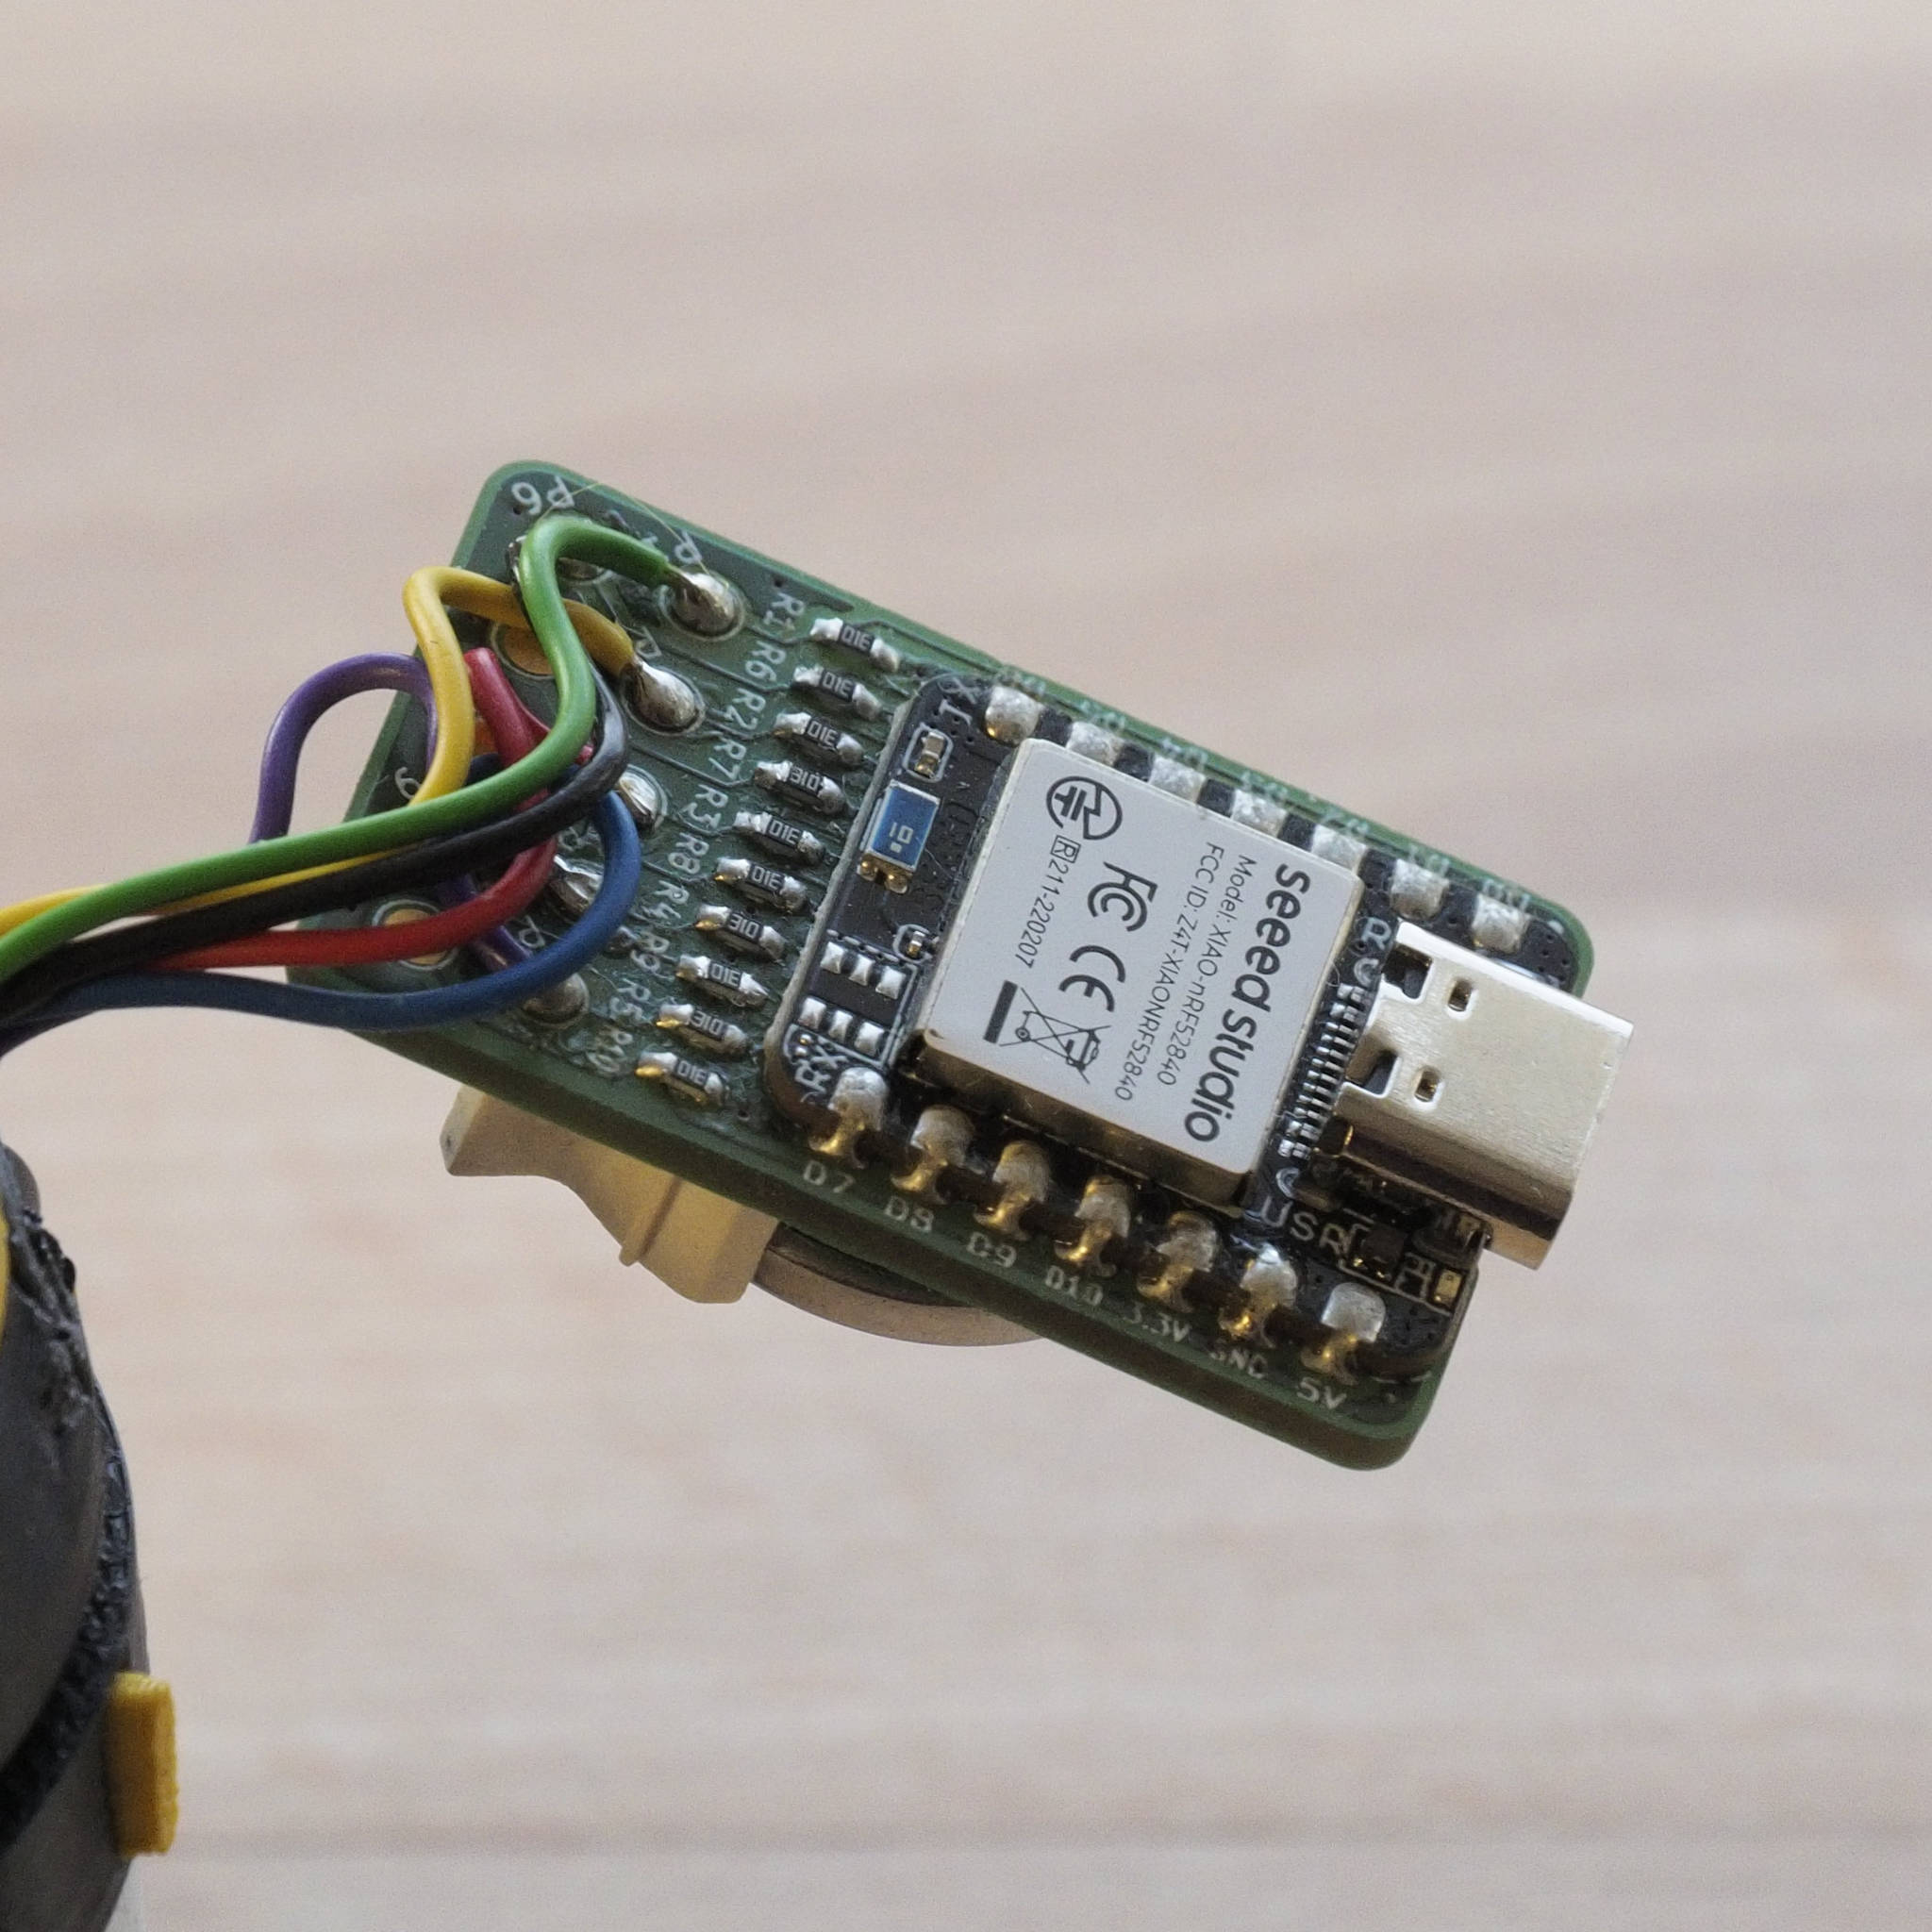
\includegraphics[width=.9\linewidth]{images/likertshift_pcb.jpg}
        \caption{Assembled PCB}
        \label{fig:likertshift_pcb}
    \end{minipage}
\end{figure}

\noindent

\subsection{Electronics}\label{subsec:electronics}

This section describes our electronics design, as well as microcontroller choice and power requirements.
For retrieving data from the prototype to our frontend (see \autoref{subsec:frontend_design}), we decided to use the Bluetooth Low Energy (BLE) network, as it offers low-power operation, is supported by most modern smartphones and does not require stationary access points to function.
We also only need very short-range communication capabilities, as the user is always situated right next to our device.

\subsubsection{Microcontroller Choice}

For data acquisition and communication we wanted to use the nRF52 series Microcontroller Units (MCUs) because of their exceptionally low-power usage, Bluetooth Low Energy (BLE) capabilities and wide availability\footnoteurl{https://docs.nordicsemi.com/category/nrf-52-series}.
Specifically, for our prototype we decided to use a relatively affordable (\ref{drq:affordable}) nRF52840 based development board by Seeed Studio\footnoteurl{https://wiki.seeedstudio.com/XIAO_BLE/}.
Using a development board allowed us to skip many electrical design challenges and to test the working principle of our prototype on a solderless breadboard.

\subsubsection{Power}

To satisfy \ref{drq:robust} and \ref{drq:easy_to_reproduce} we designed our device to be fully integrated and enclosed.
Due to the given space-constraints by our mechanical design it is only powered by a standard CR2032 button cell battery.
Under optimal conditions, it should be able to power our device for at least 1--2 years.
We did not optimize our firmware to achieve this kind of power usage though (see \ref{subsec:firmware}).

\subsubsection{Printed Circuit Board (PCB)}

To minimize wiring and to keep the electronics tightly integrated, we designed a simple breakout-PCB (see \autoref{fig:likertshift_pcb}) that holds the MCU development board and a battery holder and exposes solder pads that allow easy connection of the contactors described in \ref{subsec:mechanism}.
The solder pads allow connecting of up to ten such contactors, so it can be used with variants of the device with up to nine discrete positions.
The solder pads connect directly to the MCUs' General-Purpose Input/Output (GPIO) pins, as well as a high-impedance pull-down resistors to hold the logic state to $0V$ when not in use.

The two-layer PCB design was implemented using the KiCad Electronics Design Automation Suite (KiCad EDA) and is optimized for affordable manufacturing with design rules allowing for comparably high production tolerances.
The KiCad EDA also qualifies as FOSS.

\subsubsection{Firmware}\label{subsec:firmware}

\def\gpiohigh{\texttt{HIGH}\xspace}

When powered up, the prototype starts to advertise itself via BLE, broadcasting its name and that it is ready to accept connections.
Once a central device, the smartphone in our case, initiates a connection, the prototype hosts a Generic Attribute (GATT) server providing two services, a custom \likertshift service to retrieve the currently selected switch position and a battery service to retrieve the current battery level.
Both services each offer a one-byte characteristic that can be read by the central device.

When the \likertshift characteristic gets read, first the GPIO pin connected to the contactor at the \rotatorhead gets set to a \gpiohigh state ($\sim\SI{3.3}{V}$) then each of the pins connected to the switching contacts gets read, checking for a matching \gpiohigh state.
Finally, the detected position gets sent back to the central device, as a value from \mbox{$1$ -- $n_{positions}$}.
There are two special cases here:
\vspace*{-0.5em}
\begin{enumerate}[label=(\roman*),itemsep=0em]
    \item No switching contact is set to a \gpiohigh state.\\
        This can happen if the service gets read while the prototype is currently being moved from one position to another. In this case the service will return a value of $0$. How exactly this state should be handled is left to the software running of the central device.
    \item Multiple switching contacts are set to a \gpiohigh state.\\
        This should not happen during normal operation. In this case the service returns the position corresponding to the last GPIO pin read.
\end{enumerate}
\vspace*{-0.5em}
\noindent
When the battery characteristic gets read, the battery voltage is measured by the MCUs onboard Analog to Digital Converter (ADC).
Then, the measured voltage gets linearized and scaled to a value from $0$ -- $255$ and sent back to the central device.

\bigbreak\noindent
The firmware is written in Rust\footnoteurl{https://www.rust-lang.org/} using Embassy\footnoteurl{https://embassy.dev/} (a framework for embedded applications).

\newpage
\subsection{Frontend Design}\label{subsec:frontend_design}

To view and record ratings using the \likertshift we need a frontend that can connect to it via BLE and talk to our firmware to retrieve the currently selected position.
Because we also want to record location data simultaneously and the \likertshift hardware does not possess GPS recording capabilities, we decided to implement this frontend as a smartphone app.
This way, we can also extend it to query other information, relevant for our evaluation, from study participants.

\subsubsection{Features}

The base implementation of the app allows users to:

\begin{itemize}[itemsep=0em]
    \item connect to nearby \likertshift devices and display their currently selected rating.
    \item record GPS locations and \likertshift ratings along arbitrary travel routes.
    \item view their current location and travelled route on a 2D map.
\end{itemize}

\noindent
We later extended the app for performing our own field-study.
We took great care to make it as customizable and reusable as possible, so other researchers could reuse it to replicate our results or perform their own studies.
Thus, we added the ability for researchers to:

\begin{itemize}[itemsep=0em]
    \item inquire basic demographic information from study participants.
    \item predefine routes that participants should follow along and display them in the map view in addition to the actual travelled route.
    \item add custom surveys that appear when participants finish recording a route.
    \item record audio interviews.
    \item bundle up and export all recorded data to a single \texttt{ZIP} archive and reset the app back to a default state.
\end{itemize}

\noindent
Surveys and routes can be defined in a human-readable \texttt{JSON} format, so minimal programming knowledge is required to customize the app.
For evaluating the \likertshift in our own field-study we also added the ability to use the other recording methods described in \autoref{subsec:recording_methods}.

\subsubsection{Implementation Details}\label{subsec:implementation_details}

\def\mapscreen{\textsf{Map Screen}\xspace}
\def\routesscreen{\textsf{Routes Screen}\xspace}
\def\devicesscreen{\textsf{Devices Screen}\xspace}
\def\settingsscreen{\textsf{Settings Screen}\xspace}

The app is divided into four main screens which can be switched between by using the bottom bar.
When it gets started for the first time, the user is presented with a demographics form to fill-in (see \autoref{subfig:app_demographics_form}).
All form and survey data gets saved locally in a \texttt{JSON} format.

\begin{figure}[!htb]
    \centering
    %\captionsetup{format=plain,justification=centering,labelsep=newline}
    \begin{subfigure}{.25\textwidth}
        \centering
        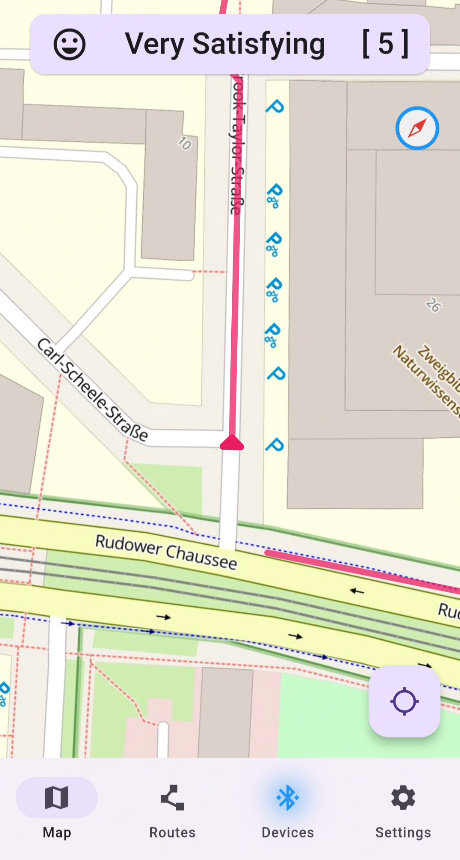
\includegraphics[width=.8666\linewidth]{images/app_map_screen.jpg}
        \caption{\mapscreen}
        \label{subfig:app_map_screen}
    \end{subfigure}%
    \begin{subfigure}{.25\textwidth}
        \centering
        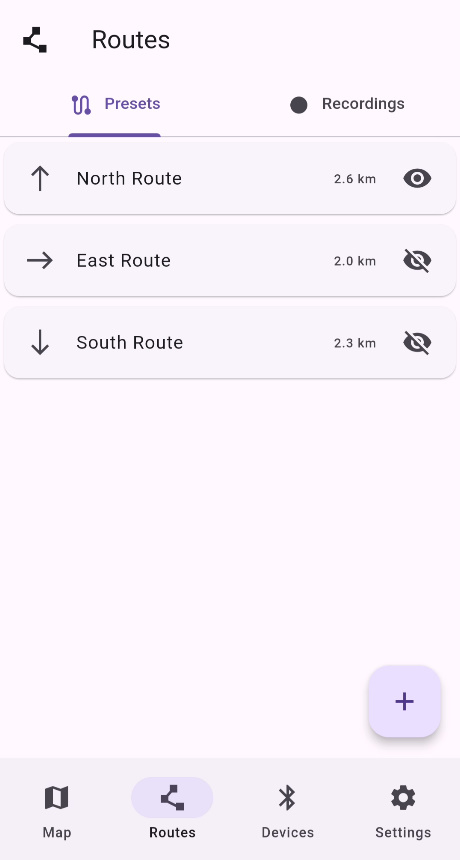
\includegraphics[width=.8666\linewidth]{images/app_routes_screen.jpg}
        \caption{\routesscreen}
        \label{subfig:app_routes_screen}
    \end{subfigure}%
    \begin{subfigure}{.25\textwidth}
        \centering
        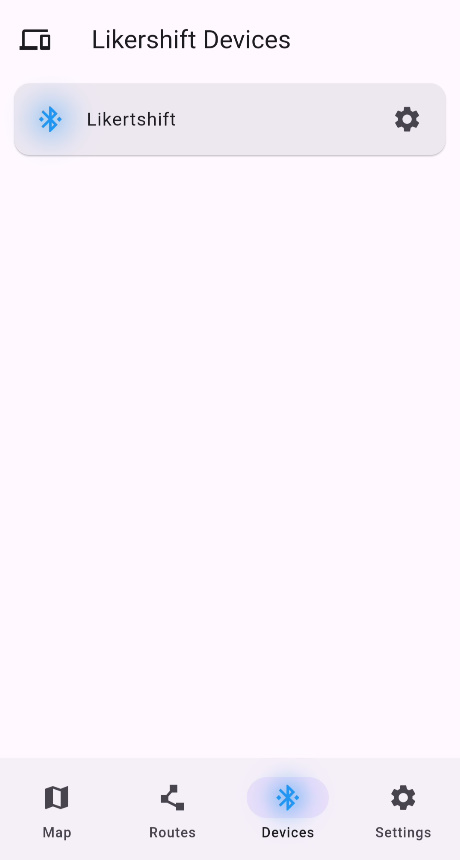
\includegraphics[width=.8666\linewidth]{images/app_devices_screen.jpg}
        \caption{\devicesscreen}
        \label{subfig:app_devices_screen}
    \end{subfigure}%
    \begin{subfigure}{.25\textwidth}
        \centering
        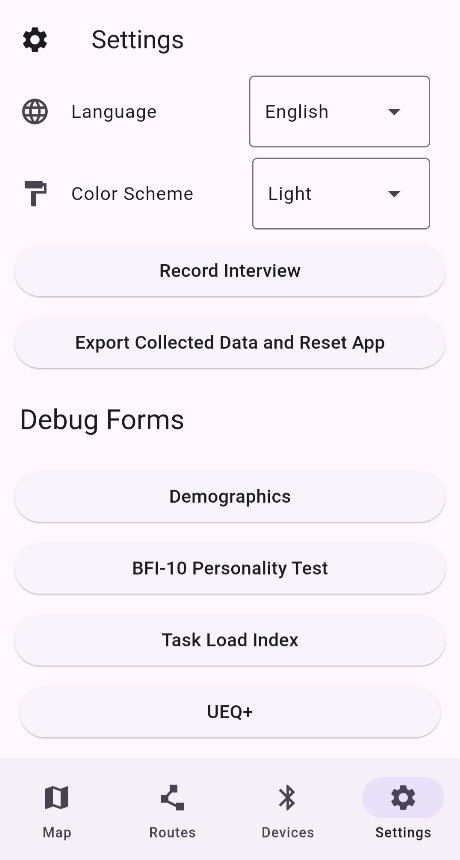
\includegraphics[width=.8666\linewidth]{images/app_settings_screen.jpg}
        \caption{\settingsscreen}
        \label{subfig:app_settings_screen}
    \end{subfigure}
    \caption{An overview of the four main app pages}
\end{figure}

\subsubsection*{Map Screen}

The \mapscreen displays the users current location and surroundings on a 2D map (see \autoref{subfig:app_map_screen}).
It can be moved and rotated using standard touch gestures.
The user can press the bottom-right toggle to make the map automatically follow the current location and long-press the compass to lock the rotation to the current movement direction.
If the user starts a recording, the \mapscreen will also display the travelled route, as well as the preset route, if one was selected.
Additionally, if a \likertshift device is connected, the \mapscreen will also display the devices' currently selected numeric rating and a description of its meaning.
Routes from the \routesscreen can also be previewed on the \mapscreen.

\subsubsection*{Routes Screen and Route Recording}

The \routesscreen is divided into two tabs, showing the available route presets and past recordings respectively (see \autoref{subfig:app_routes_screen}).
Route presets can be previewed using the “Eye” buttons and new recordings can be started using the \raisebox{0.1em}{\textbf{+}} button.

When starting a new recording the user has to select a recording method and optionally a route preset.
Then, whenever the app receives a location update (every $\sim1$--$\SI{5}{s}$), a new data point will be added to the recording, containing the new location, the time elapsed since starting the recording and the current rating value by the active \likertshift device, if available.
This data is then immediately written to a new line in a \texttt{CSV} file, to prevent data loss in case of app crashes or battery run out.
A recording can be stopped at any time by pressing the “Stop Recording” button that will appear above the main navigation bar.
Once a recording is finished, the user can be presented with various forms and surveys (see \autoref{subfig:app_tlx_survey} for an example we used in our field-study).

\subsubsection*{Devices Screen}

The \devicesscreen allows discovering of and connecting to nearby \likertshift devices (see \autoref{subfig:app_devices_screen}).
It displays a list of currently advertising and already known devices.
A new connection can be established by selecting one of the devices from the list.
Only one device can be connected to at any time.
If a connection gets established successfully, its Bluetooth icon lights up, signaling that its currently connected.
During connection, the \likertshift device is queried for its currently selected rating value every \SI{500}{ms} (this update rate can be easily adjusted).
Invalid ratings (see \autoref{subsec:firmware}) are ignored, so the previous rating is kept.

\subsubsection*{Settings Screen}

The apps' language and color theme can be adjusted in the \settingsscreen (see \autoref{subfig:app_settings_screen}).
It has been fully translated to English and German for use in our field-study.
Additionally, it allows navigating to the \textsf{Interview Recording Screen}, which offers a simple interface to start, pause and stop recording an audio interview (see \autoref{subfig:app_interview_recorder}).
Recorded audio interviews will also be saved locally as losslessly encoded \texttt{FLAC} files.
Finally, the \settingsscreen offers a button to “Export collected Data and Reset the App” which will bundle all recorded data into a single \texttt{ZIP} file and store it locally, under a randomly generated participant ID.
Said ID will then be reported back to the user, and the app will be reset (see \autoref{subfig:app_data_export}).

\begin{figure}[!htb]
    \centering
    \begin{subfigure}{.25\textwidth}
        \centering
        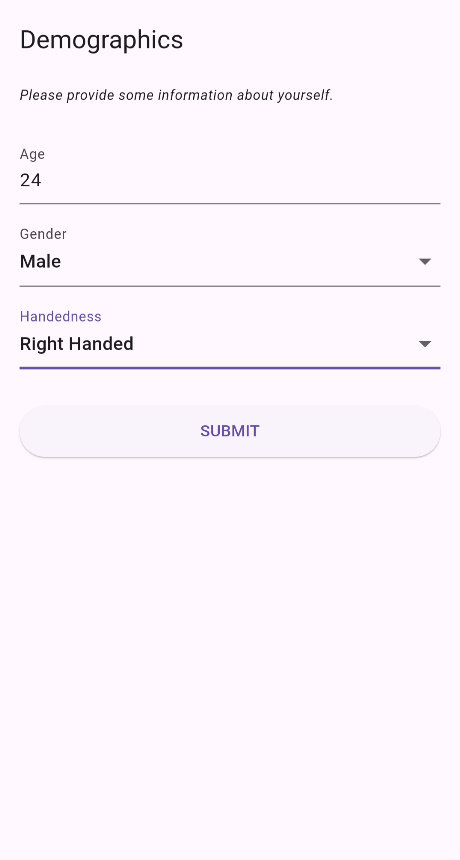
\includegraphics[width=.8666\linewidth]{images/app_demographics_form.jpg}
        \caption{Demographics form}
        \label{subfig:app_demographics_form}
    \end{subfigure}%
    \begin{subfigure}{.25\textwidth}
        \centering
        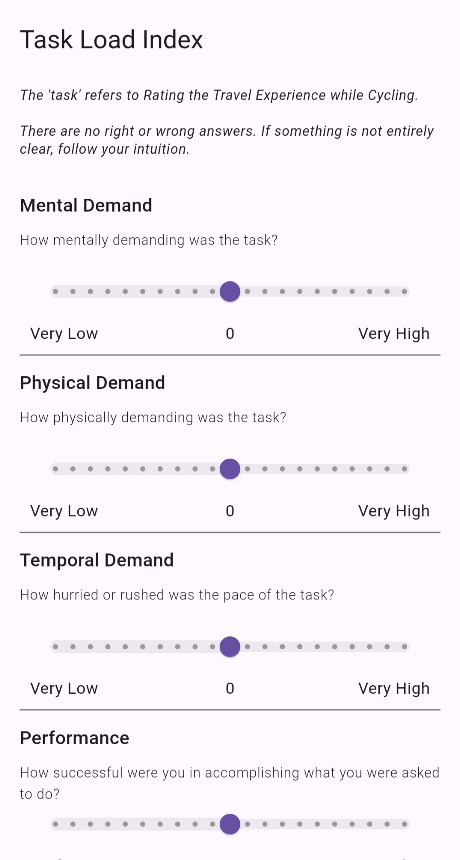
\includegraphics[width=.8666\linewidth]{images/app_tlx_survey.jpg}
        \caption{TLX survey}
        \label{subfig:app_tlx_survey}
    \end{subfigure}%
    \begin{subfigure}{.25\textwidth}
        \centering
        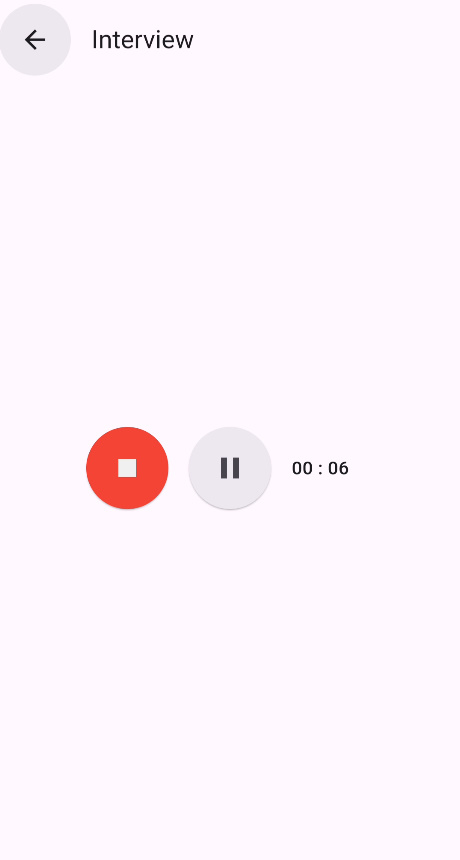
\includegraphics[width=.8666\linewidth]{images/app_interview_recorder.jpg}
        \caption{Interview recorder}
        \label{subfig:app_interview_recorder}
    \end{subfigure}%
    \begin{subfigure}{.25\textwidth}
        \centering
        
\includegraphics[width=.8666\linewidth]{images/app_reset_screen.jpg}
        \caption{Data export}
        \label{subfig:app_data_export}
    \end{subfigure}
    \caption{Contextual screens}
\end{figure}

\noindent
The app is written using the Flutter\footnoteurl{https://flutter.dev/} framework and Dart\footnoteurl{https://dart.dev/} programming language.
While we only tested and used our app on Android devices, the multi-platform nature of Flutter should also allow it to run on iOS powered devices with minimal modifications.
